\chapter{TINJAUAN PUSTAKA}

\section{Kanker}

    Kanker merupakan pertumbuhan sel yang tidak terkendali pada organ tubuh manusia dan dapat menyebar ke dalam organ tubuh lainnya. Perubahan sel normal menjadi sel kanker disebut sebagai karsinogenesis yang terdiri dari tiga tahap. Tahap pertama merupakan tahap inisiasi yang mengubah ekspresi gen atau bahkan penghapusan bagian DNA akibat mutasi gen. Tahap kedua merupakan tahap promosi yang memulai sel-sel berproliferasi. Tahap terakhir merupakan tahap progresif yang memulai perkembangan sel secara agresif dengan pada jumlah dan ukuran sehingga membentuk tumor primer. Pada tahap ini, sel melakukan invasi dan mulai bermetastasis \citep{Baranwal2021}.

    Ketika sel bertumbuh di luar batas normal dan tidak mengalami kematian, maka akan membentuk tumor \citep{Shedden-Mora2020}. Terdapat dua jenis tumor, yaitu \textit{benign} (tumor jinak) dan \textit{malignant} (tumor ganas). \textit{Benign} tumbuh dengan lambat dan tidak menyebar pada jaringan di sekitarnya. \textit{Benign} tidak berbahaya terhadap tubuh manusia dan prognosisnya baik \citep{Wu2021b}. Sedangkan \textit{malignant} berkembang dan tumbuh serta mengganggu jaringan di sekitarnya. Menghilangkan tumor cenderung sulit meskipun dengan pembedahan. Karena \textit{malignant} tidak berdiferensiasi dengan baik dan tidak matang sehingga menyebar ke dalam jaringan di sekitarnya \citep{li2022epidemiology}. Akibatnya, sering terjadi pertumbuhan tumor lagi setelah pembedahan. Metastasis sering terjadi karena menyebar ke dalam jaringan di sekitarnya. Jika tidak dilakukan pembedahan, terapi radiasi, atau terapi kemo maka akan mengakibatkan kematian. Terkait \textit{malignant}, prognosis bergantung pada waktu diagnosis, derajat kemajuan, dan metastasis \citep{Park2022}.

    Terdapat beberapa penanganan medis untuk mengatasi sel kanker yang berkembang, yaitu pembedahan, terapi kemo, terapi hormon, terapi biologis, dan terapi radiasi. Pembedahan dilakukan oleh tenaga medis dengan memotong sel kanker. Terapi kemo merupakan penanganan sel kanker dengan pemberian obat untuk membunuh sel kanker \citep{Strobel2019}. Terapi hormon digunakan untuk menghentikan hormon yang dibutuhkan oleh sel kanker dalam berkembang. Terapi biologis bekerja dengan sistem kekebalan tubuh untuk menangani sel kanker atau menangani efek samping dari sel kanker \citep{Waks2019}. Terapi radiasi menggunakan sinar-X untuk membunuh sel kanker \citep{Wu2021}. Akan tetapi, berbagai metode tersebut belum tentu sesuai untuk setiap orang dan terdapat efek samping dalam melakukan setiap metode tersebut.

\section{Kanker Kulit}
Kanker kulit merupakan penyakit yang mengubah sel normal pada kulit menjadi sel kanker. Sel kanker akan tumbuh pada kulit secara terus menerus dan biasanya tidak simetris. Kanker kulit memiliki struktur yang tidak umum dengan diferensiasi sel pada tingkat kromatin, nukleus, dan sitoplasma. Hal ini karena terdapat kerusakan pada DNA. Kerusakan pada DNA dapat terjadi karena paparan sinar UV secara berlebihan. Radiasi sinar UV dapat menembus bagian dalam kulit sehingga dapat membunuh sel-sel kulit termasuk DNA pada sel. Kerusakan pada DNA dapat menyebabkan malfungsi sehingga DNA pada sel bermutasi \citep{Nugroho2019}.

    \subsection{\textit{Melanoma} (MEL)}
    MEL termasuk dalam kanker kulit yang sangat berbahaya. Kanker kulit MEL dapat menyebar ke dalam organ tubuh lain. MEL berasal dari melanosit. Melanosit merupakan sel penghasil melanin yang ada pada kulit. MEL memiliki bentuk yang tidak normal, tidak simetris, dan memiliki lebih dari satu warna. Tahi lalat yang terkena MEL dapat menimbulkan rasa gatal dan mengeluarkan darah. MEL biasanya ditemukan di vulva, mata, kulit, sinus, paru-paru, tenggorokan, saluran pencernaan, dan saluran reproduksi. Selain itu, kanker kulit MEL juga dapat ditemukan di bagian anus dan rektum. MEL lebih sering ditemukan di tubuh seorang pria daripada seorang wanita. Hampir sama dengan jenis kanker kulit lain, penyebab utama kemunculan kanker kulit MEL karena mutasi genetik akibat radiasi sinar UV. Sinar UV tidak merusak DNA secara langsung, akan tetapi membentuk spesies oksigen reaktif sepanjang fotoreseptor non-DNA pada tubuh. Radikal oksigen yang dihasilkan menyebabkan kerusakan dan fragmentasi DNA sehingga mengakibatkan mutasi gen \citep{Sang2019}. Kanker kulit MEL seperti terlihat pada Gambar \ref{fig:mel}.
    \begin{figure}[H] 
        \begin{center} 
            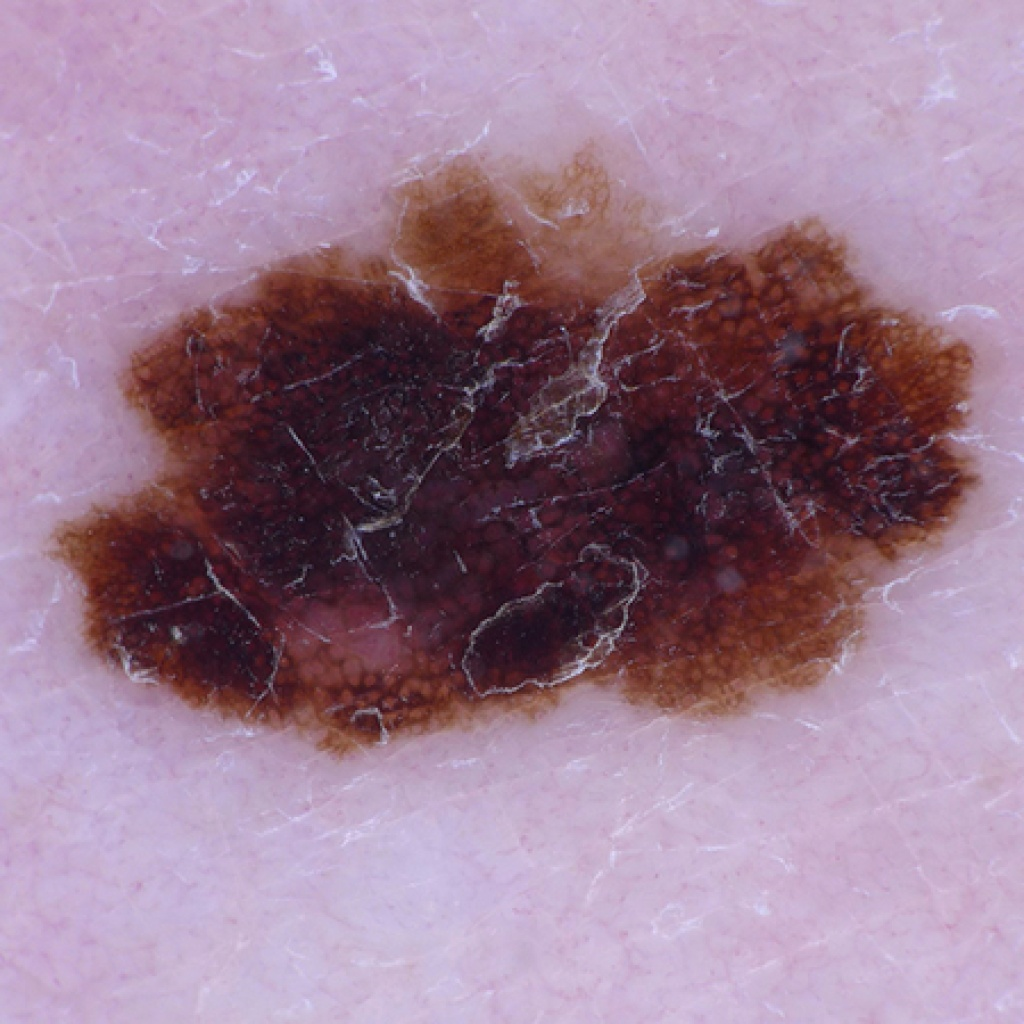
\includegraphics[width=4cm]{../img/Skin Cancer MEL - Latex.jpg}
            \caption{Kanker kulit MEL} 
            \label{fig:mel}
            Sumber: \citep{Codella2018,Combalia2019,Tschandl2018}
        \end{center} 
    \end{figure}

    \subsection{\textit{Actinic Keratosis} (AK)}
    AK merupakan kanker kulit yang sangat umum diderita. Paparan sinar UV yang sangat tinggi pada tubuh dapat menyebabkan kemunculan AK, seperti pada bagian wajah, kulit kepala, leher, punggung tangan, dan lengan. AK memiliki kemungkinan berevolusi menjadi SCC, akan tetapi tidak memungkinkan untuk memprediksi setiap lesi. Oleh karena itu, pengobatan AK sangat penting untuk menghindari perubahannya menjadi SCC. Seseorang yang berusia lebih dari 40 tahun memiliki kecenderungan untuk terkena AK daripada seseorang yang lebih muda \citep{Dianzani2020}. Kanker kulit actinic keratosis seperti terlihat pada Gambar \ref{fig:ak}.
    \begin{figure}[H] 
        \begin{center} 
            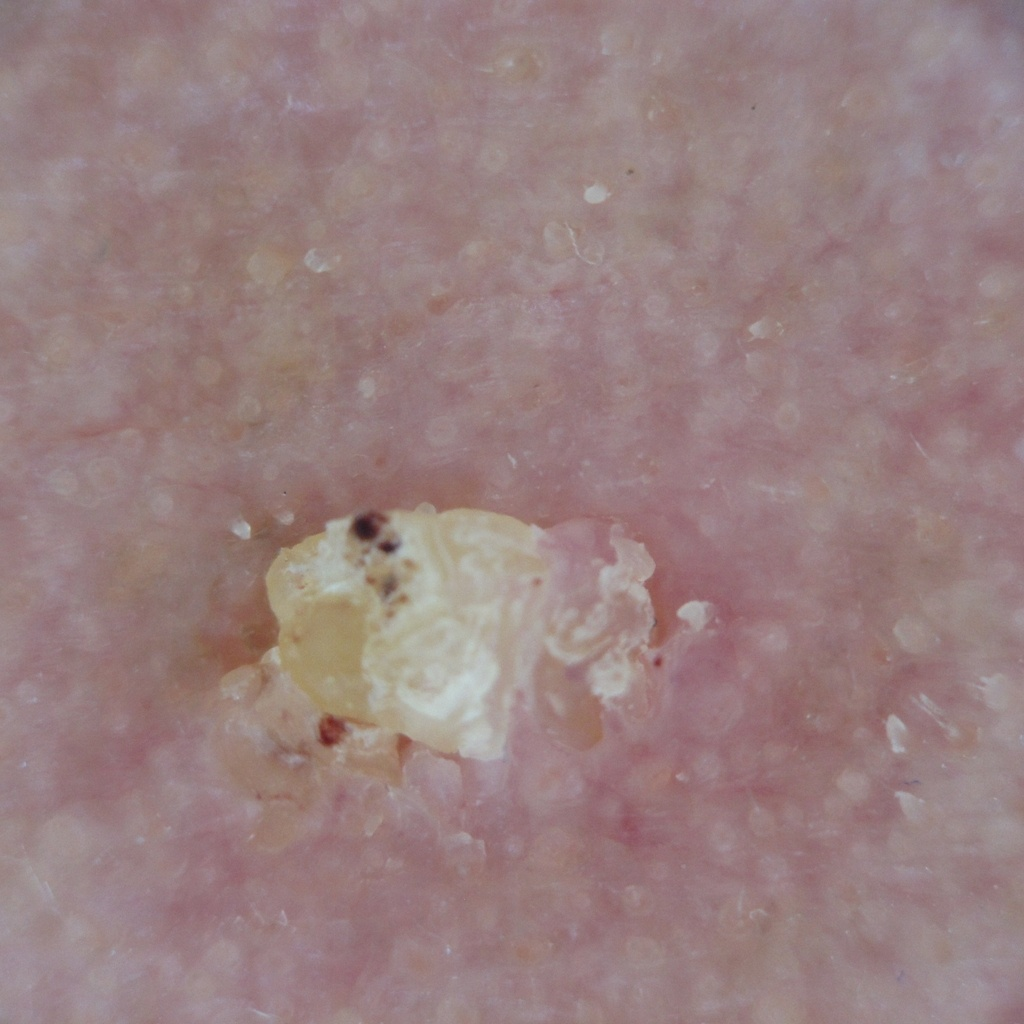
\includegraphics[width=4cm]{../img/Skin Cancer AK - Latex.jpg}
            \caption{Kanker kulit AK} 
            \label{fig:ak}
            Sumber: \citep{Codella2018,Combalia2019,Tschandl2018}
        \end{center} 
    \end{figure}

    \subsection{\textit{Melanocytic Nevus} (NV)}
    NV merupakan benign yang berasal dari melanosit, sel dendritik yang menghasilkan pigmen, dan biasanya ditemukan di antara keratinosit yang berada pada lapisan basal epidermis. NV yang bertumbuh sangat berbahaya karena berpotensi menjadi melanoma. NV memiliki ciri-ciri seperti tahi lalat. Jika NV sering terpapar polusi, sinar UV, dan bahan kimia berbahaya dapat berpotensi menjadi melanoma. Kanker kulit jenis ini memberikan efek bagi seseorang yang terkena komplikasi, seperti gangguan saraf, kejang, pingsan, dan muntah \citep{Fuadah2020a}. Kanker kulit nevus seperti terlihat pada Gambar \ref{fig:nv}.
    \begin{figure}[H] 
        \begin{center} 
            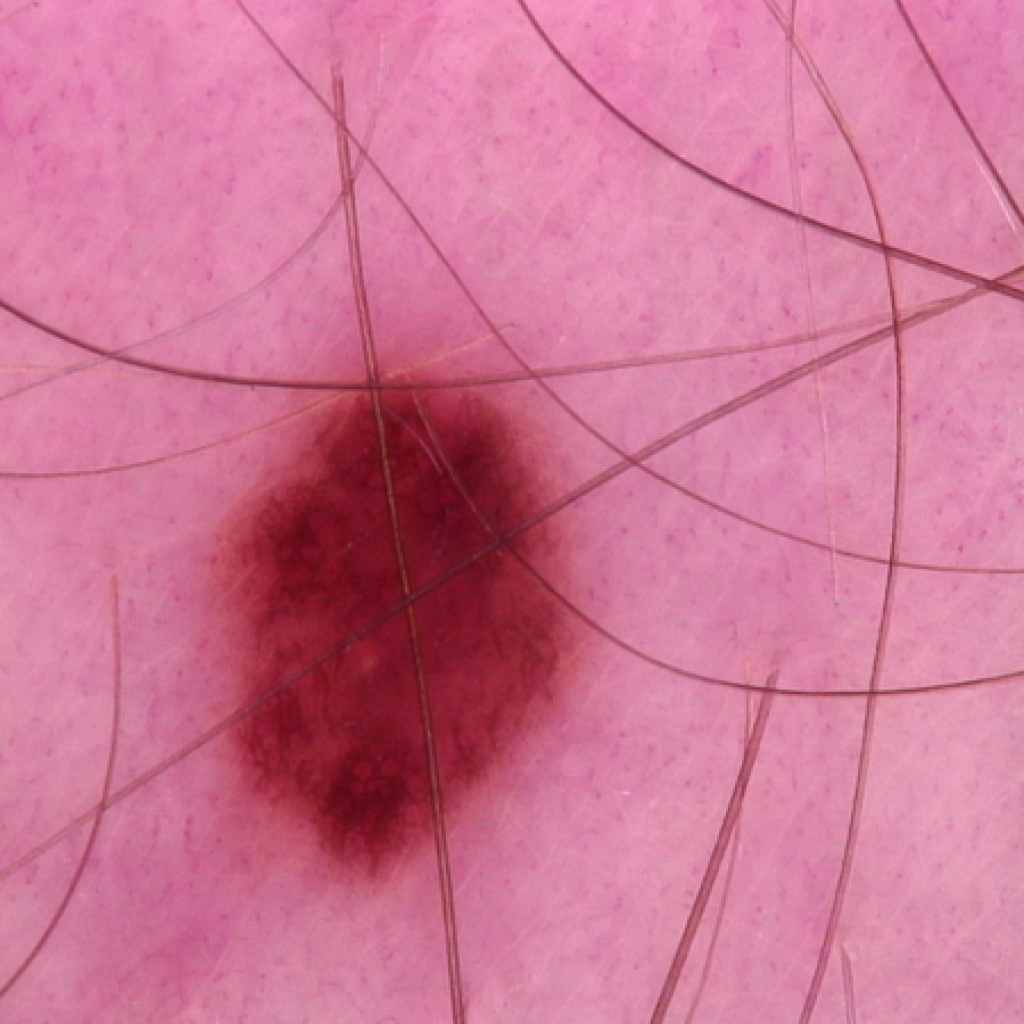
\includegraphics[width=4cm]{../img/Skin Cancer NV - Latex.jpg}
            \caption{Kanker kulit NV} 
            \label{fig:nv}
            Sumber: \citep{Codella2018,Combalia2019,Tschandl2018}
        \end{center} 
    \end{figure}

    \subsection{\textit{Basal Cell Carcinoma} (BCC)}
    BCC merupakan kanker kulit yang dari sel-sel basal di dekat persimpangan epidermis-dermis. Kanker kulit jenis ini tumbuh dengan lambat dan tidak bermigrasi. Kemunculan BCC seringkali karena paparan sinar matahari secara langsung dan berlebihan dan biasanya terdapat pada bagian wajah atau leher. Pria dan orang yang semakin tua memiliki presentase lebih tinggi untuk terkena BCC. Diet energi tinggi (khususnya lemak tinggi, vitamin rendah), bahan kimia berbahaya, dan paparan debu juga dapat menyebabkan munculnya BCC. Dalam praktiknya, BCC dibagi menjadi empat jenis, yaitu jenis dangkal, nodular, pigmen, dan titik keras \citep{Sang2019}. Kanker kulit BCC seperti terlihat pada Gambar \ref{fig:bcc}.
    \begin{figure}[H] 
        \begin{center} 
            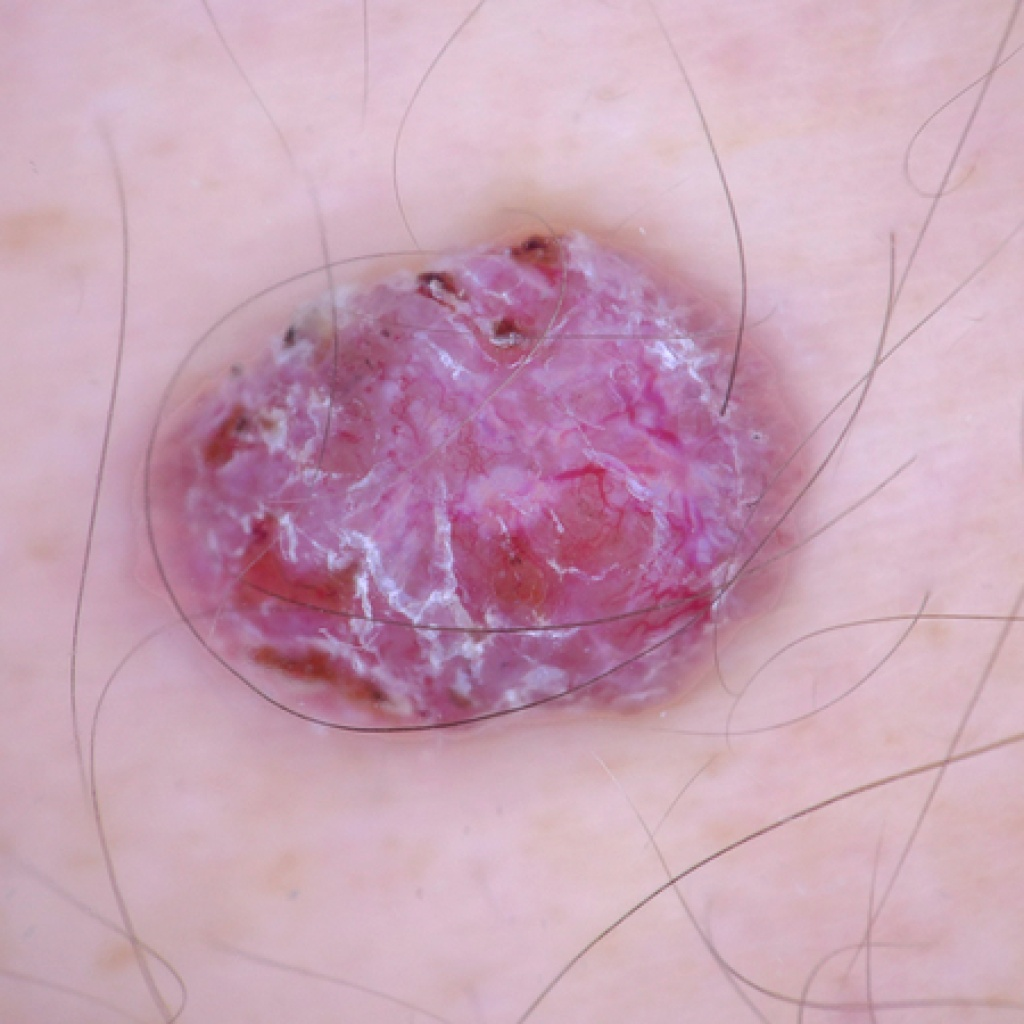
\includegraphics[width=4cm]{../img/Skin Cancer BCC - Latex.jpg}
            \caption{Kanker kulit BCC} 
            \label{fig:bcc}
            Sumber: \citep{Codella2018,Combalia2019,Tschandl2018}
        \end{center} 
    \end{figure}

    \subsection{\textit{Squamous Cell Carcinoma} (SCC)}
    SCC merupakan tipe kanker kulit yang tidak agresif. Kanker kulit jenis ini tumbuh dengan lambat. Terapi tanpa pembedahan dapat menangani SCC jika didiagnosis lebih awal. Karena benign dapat bertumbuh dengan terus menerus serta menyebar ke tulang, jaringan, dan bahkan kelenjar getah bening jika tidak ditangani sejak awal \citep{Fuadah2020a}. SCC kebanyakan diderita oleh seseorang yang berusia lebih dari 60 tahun dan berjenis kelamin pria. Daerah invasi SCC dapat dibagi menjadi tiga bagian, yaitu dangkal, dalam, dan tipe transfer \citep{Sang2019}. Kanker kulit SCC seperti terlihat pada Gambar \ref{fig:scc}.
    \begin{figure}[H] 
        \begin{center} 
            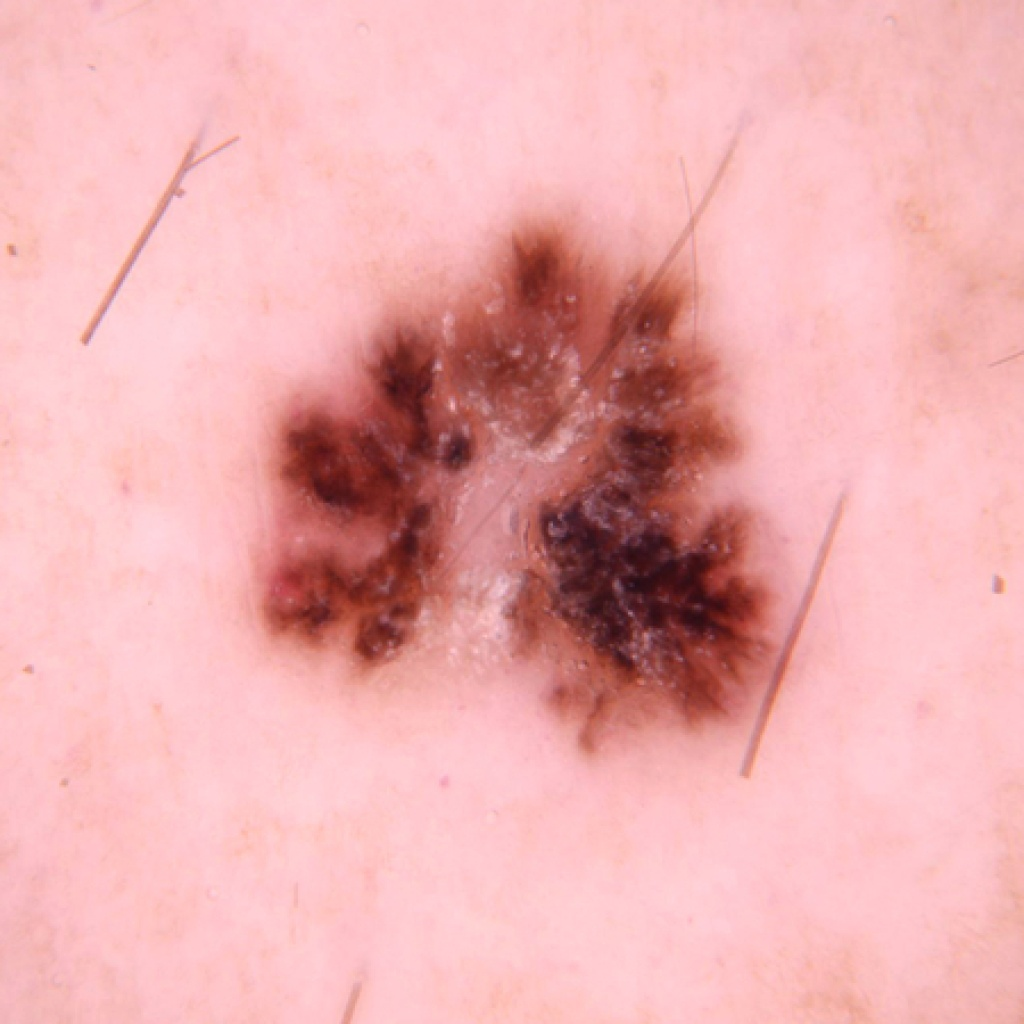
\includegraphics[width=4cm]{../img/Skin Cancer SCC - Latex.jpg}
            \caption{Kanker kulit SCC} 
            \label{fig:scc}
            Sumber: \citep{Codella2018,Combalia2019,Tschandl2018}
        \end{center} 
    \end{figure}

    \subsection{\textit{Dermatofibroma} (DF)}
    DF termasuk ke dalam kategori benign. Kanker kulit jenis ini muncul karena pertumbuhan campuran dari jenis sel di lapisan dermis kulit secara berlebih. Gejala defmatofibroma muncul setelah mengalami beberapa trauma kulit ringan, seperti luka tusuk. Dermatofibroma berukuran sekitar 2-3 mm, berwarna coklat keunguan, berstruktur keras, dan menimbulkan rasa nyeri ketika ditekan \citep{Fuadah2020a}. Kanker kulit DF seperti terlihat pada Gambar \ref{fig:df}.
    \begin{figure}[H] 
        \begin{center} 
            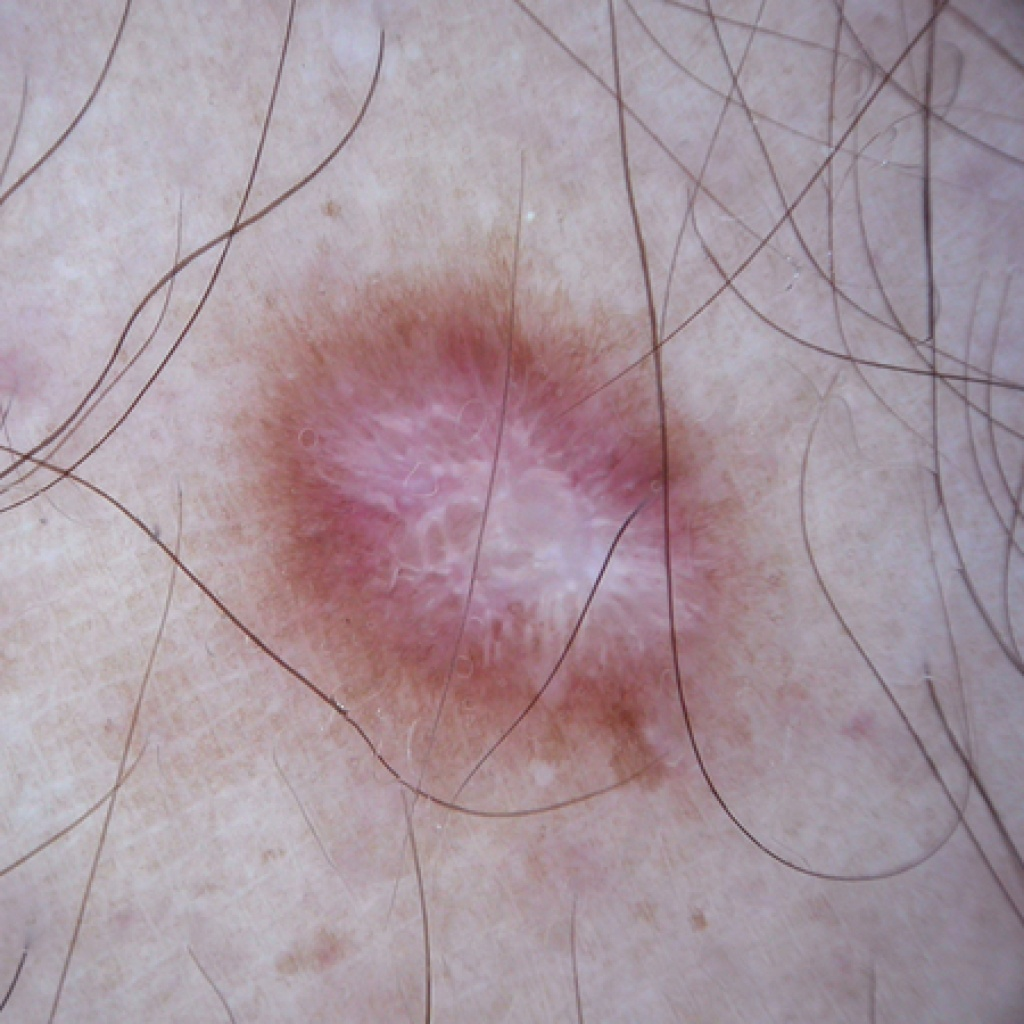
\includegraphics[width=4cm]{../img/Skin Cancer DF - Latex.jpg}
            \caption{Kanker kulit DF} 
            \label{fig:df}
            Sumber: \citep{Codella2018,Combalia2019,Tschandl2018}
        \end{center} 
    \end{figure}

    \subsection{\textit{Benign Keratosis Lesion} (BKL)}
    BKL merupakan kanker kulit yang tidak berbahaya dan tumbuh dengan warna coklat, hitam, atau coklat lilin. BKL cenderung tidak berbahaya dan tidak memerlukan perawatan khusus. Tampilan umum dari BKL berupa bercak bulat atau oval yang seakan-akan menempel pada kulit. Kanker kulit jenis ini lebih sering terjadi seiring bertambahnya usia. Daerah kulit yang mengandung rambut dan mukosa sering kali menjadi tempat tumbuhnya BKL. Kanker kulit jenis ini juga ditemukan di daerah genital pria \citep{Hall2019}. Kanker kulit BKL seperti terlihat pada Gambar \ref{fig:bkl}.
    \begin{figure}[H] 
        \begin{center} 
            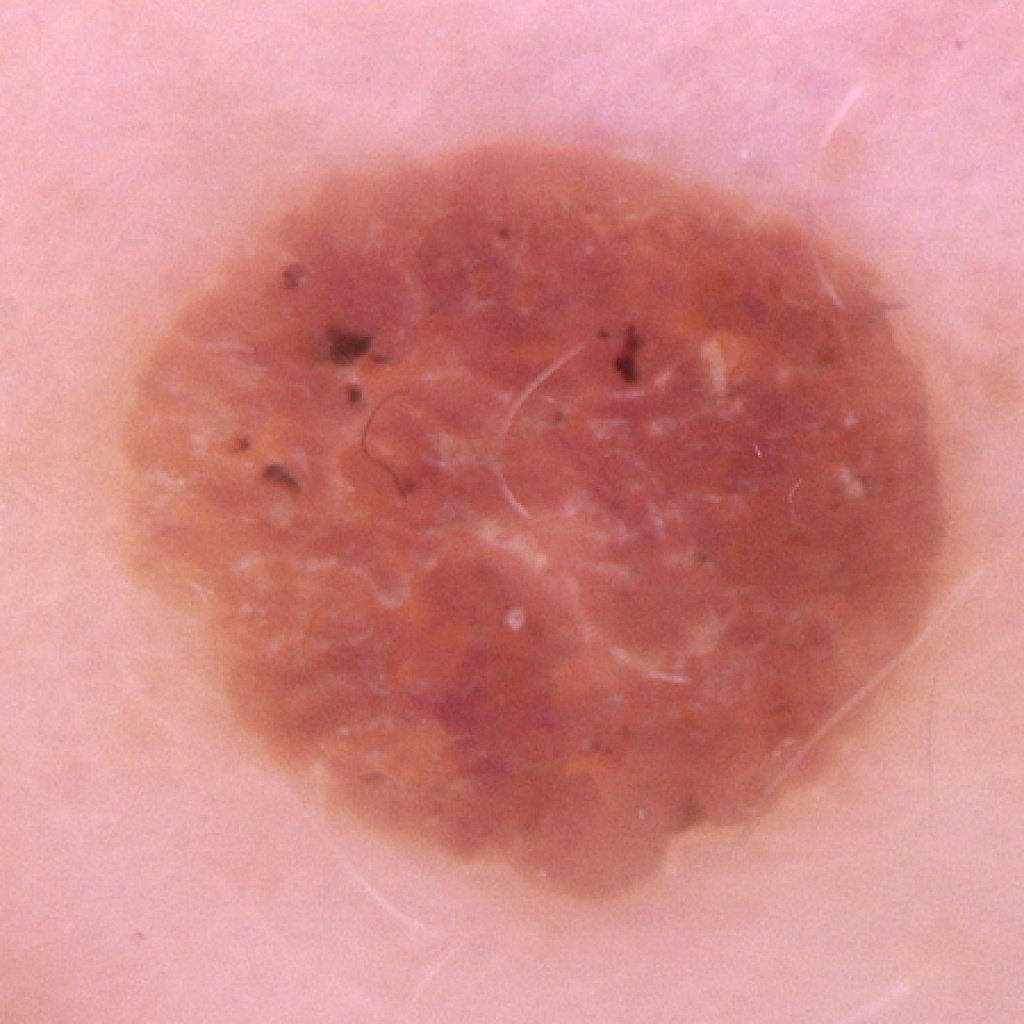
\includegraphics[width=4cm]{../img/Skin Cancer BKL - Latex.jpg}
            \caption{Kanker kulit BKL} 
            \label{fig:bkl}
            Sumber: \citep{Codella2018,Combalia2019,Tschandl2018}
        \end{center} 
    \end{figure}

    \subsection{\textit{Vascular Lesion} (VASC)}
    VASC atau yang lebih dikenal sebagai tanda lahir merupakan kanker kulit yang ada pada kulit dan jaringan di bawahnya \citep{Balas2018}. Kanker kulit jenis ini relatif umum terjadi. Terdapat tiga kategori utama dari VASC, yaitu Hemangioma, Malformasi Vaskular, dan Granuloma Piogenik. Ketiga jenis tanda lahir ini terlihat serupa, meskipun ketiganya memiliki perawatan yang berbeda-beda. Hemangioma merupakan jenis kanker kulit yang umum pada anak-anak. Seringkali Hemangioma dapat dipantau oleh dokter kulit atau dokter anak karena kanker kulit jenis ini tumbuh secara alami dan tanpa perawatan. Meskipun tidak banyak Hemangioma yang perlu perawatan khusus karena berada pada daerah yang tidak tepat. Malformasi vaskular merupakan kesalahan kongenital dalam pembentukan pembuluh darah. Malformasi vaskular memerlukan perawatan khusus karena terkait dengan kesalahan fungsi pada pembuluh darah. Granuloma piogenik merupakan kanker kulit tidak berbahaya yang terbentuk sebagai respon terhadap cedera jaringan lokal. Kanker kulit jenis ini umumnya muncul pada anak-anak dan ibu hamil pada daerah mulut dan ujung jari \citep{Rastogi2020}. Kanker kulit VASC seperti terlihat pada Gambar \ref{fig:vasc}.
    \begin{figure}[H] 
        \begin{center} 
            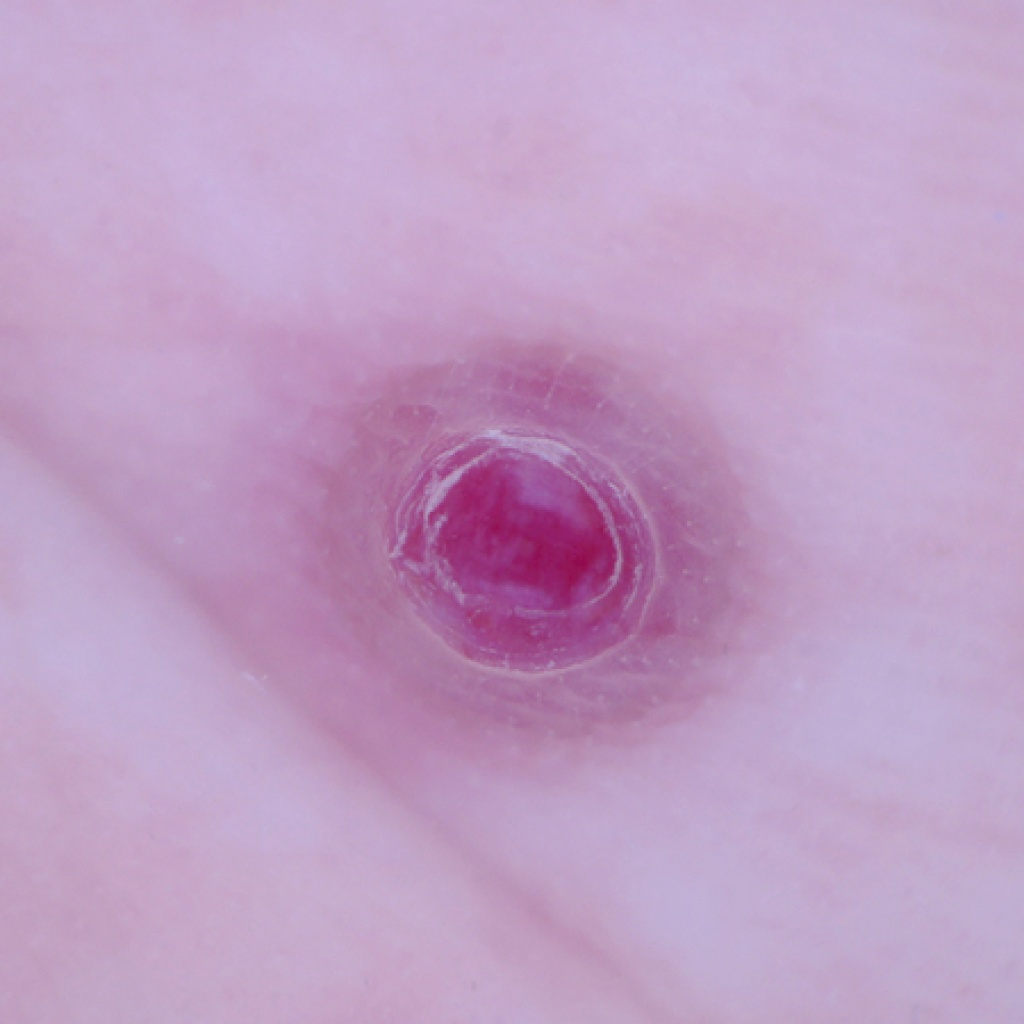
\includegraphics[width=4cm]{../img/Skin Cancer VASC - Latex.jpg}
            \caption{Kanker kulit VASC} 
            \label{fig:vasc}
            Sumber: \citep{Codella2018,Combalia2019,Tschandl2018}
        \end{center} 
    \end{figure}

\section{Citra Digital}
Sebagian besar informasi didapatkan dalam bentuk gelombak elektrik dan sinyal. Informasi dapat diubah ke dalam bentuk sinyal dua dimensi atau biasa disebut sebagai citra. Citra digital merupakan representasi dari fungsi intensitas cahaya dalam bentuk distkit pada ruang dua dimensi. Pada citra digital terdapat beberapa elemen baris dan kolom yang disebut piksel. Piksel pada citra memiliki atribut koordinat $(x,y)$ dan amplitudo $(x,y)$. Koordinat $(x,y)$ merepresentasikan letak piksel dalam sebuah citra digital. Sedangkan amplitudo $(x,y)$ menunjukkan intensitas warna yang ada pada citra \citep{Ratna2020}. Sebuah citra digital dapat dilihat sebagai gambaran visual dari matriks yang berisi bilangan bulat (integer). Bilangan bulat tersebut menunjukkan derajat keabuan untuk citra tingkat abu-abu dan menunjukkan warna untuk citra tingkat warna \citep{Blackledge2005,Septiaji2018}.

Citra dapat direpresentasikan sebagai fungsi dari dua variabel $f(x,y)$ berdasarkan tingkat keabuan $(x,y)$. Sehingga citra tersebut dapat diubah menjadi fungsi diskrit sebagai citra digital seperti terlihat pada Persamaan (\ref{eq:citra}).

\begin{align}
    f_{ij} \textnormal{ dimana } f_{ij} &\equiv f(x_i, y_i)
    \label{eq:citra}
\end{align}

$f_{ij}$ merupakan nilai fungsi pada $x=x_i$ dan $y=y_i$ sehingga bisa didefinisikan sebagai matriks atau \textit{array} dua dimensi seperti pada Persamaan \ref{eq:citra2}.

\begin{align}
    f_{ij} &=
    \begin{bmatrix}
        f_{11} &f_{12} &\cdots &f_{1n}\\
        f_{21} &f_{12} &\cdots &f_{1n}\\
        \vdots &\vdots &\ddots &\vdots\\
        f_{n1} &f_{n2} &\cdots &f_{nn}\\
    \end{bmatrix}
    \label{eq:citra2}
\end{align}

    \subsection{Citra Warna}
    Citra RGB merupakan citra digital yang memiliki tiga kanal warna, yaitu \textit{Red}, \textit{Green}, \textit{Blue} (RGB). Setiap lapisan warna, masing-masing memiliki nilai piksel antara $0$ sampai $255$. Pada umumnya, nilai piksel ini tersimpan pada memori komputer atau berkas tertentu dalam bentuk 8-bit atau $2^8$ warna. Gambar \ref{fig:color} merupakan contoh citra RGB \citep{Septiaji2018}.

    \begin{figure}[H]
        \begin{center}
            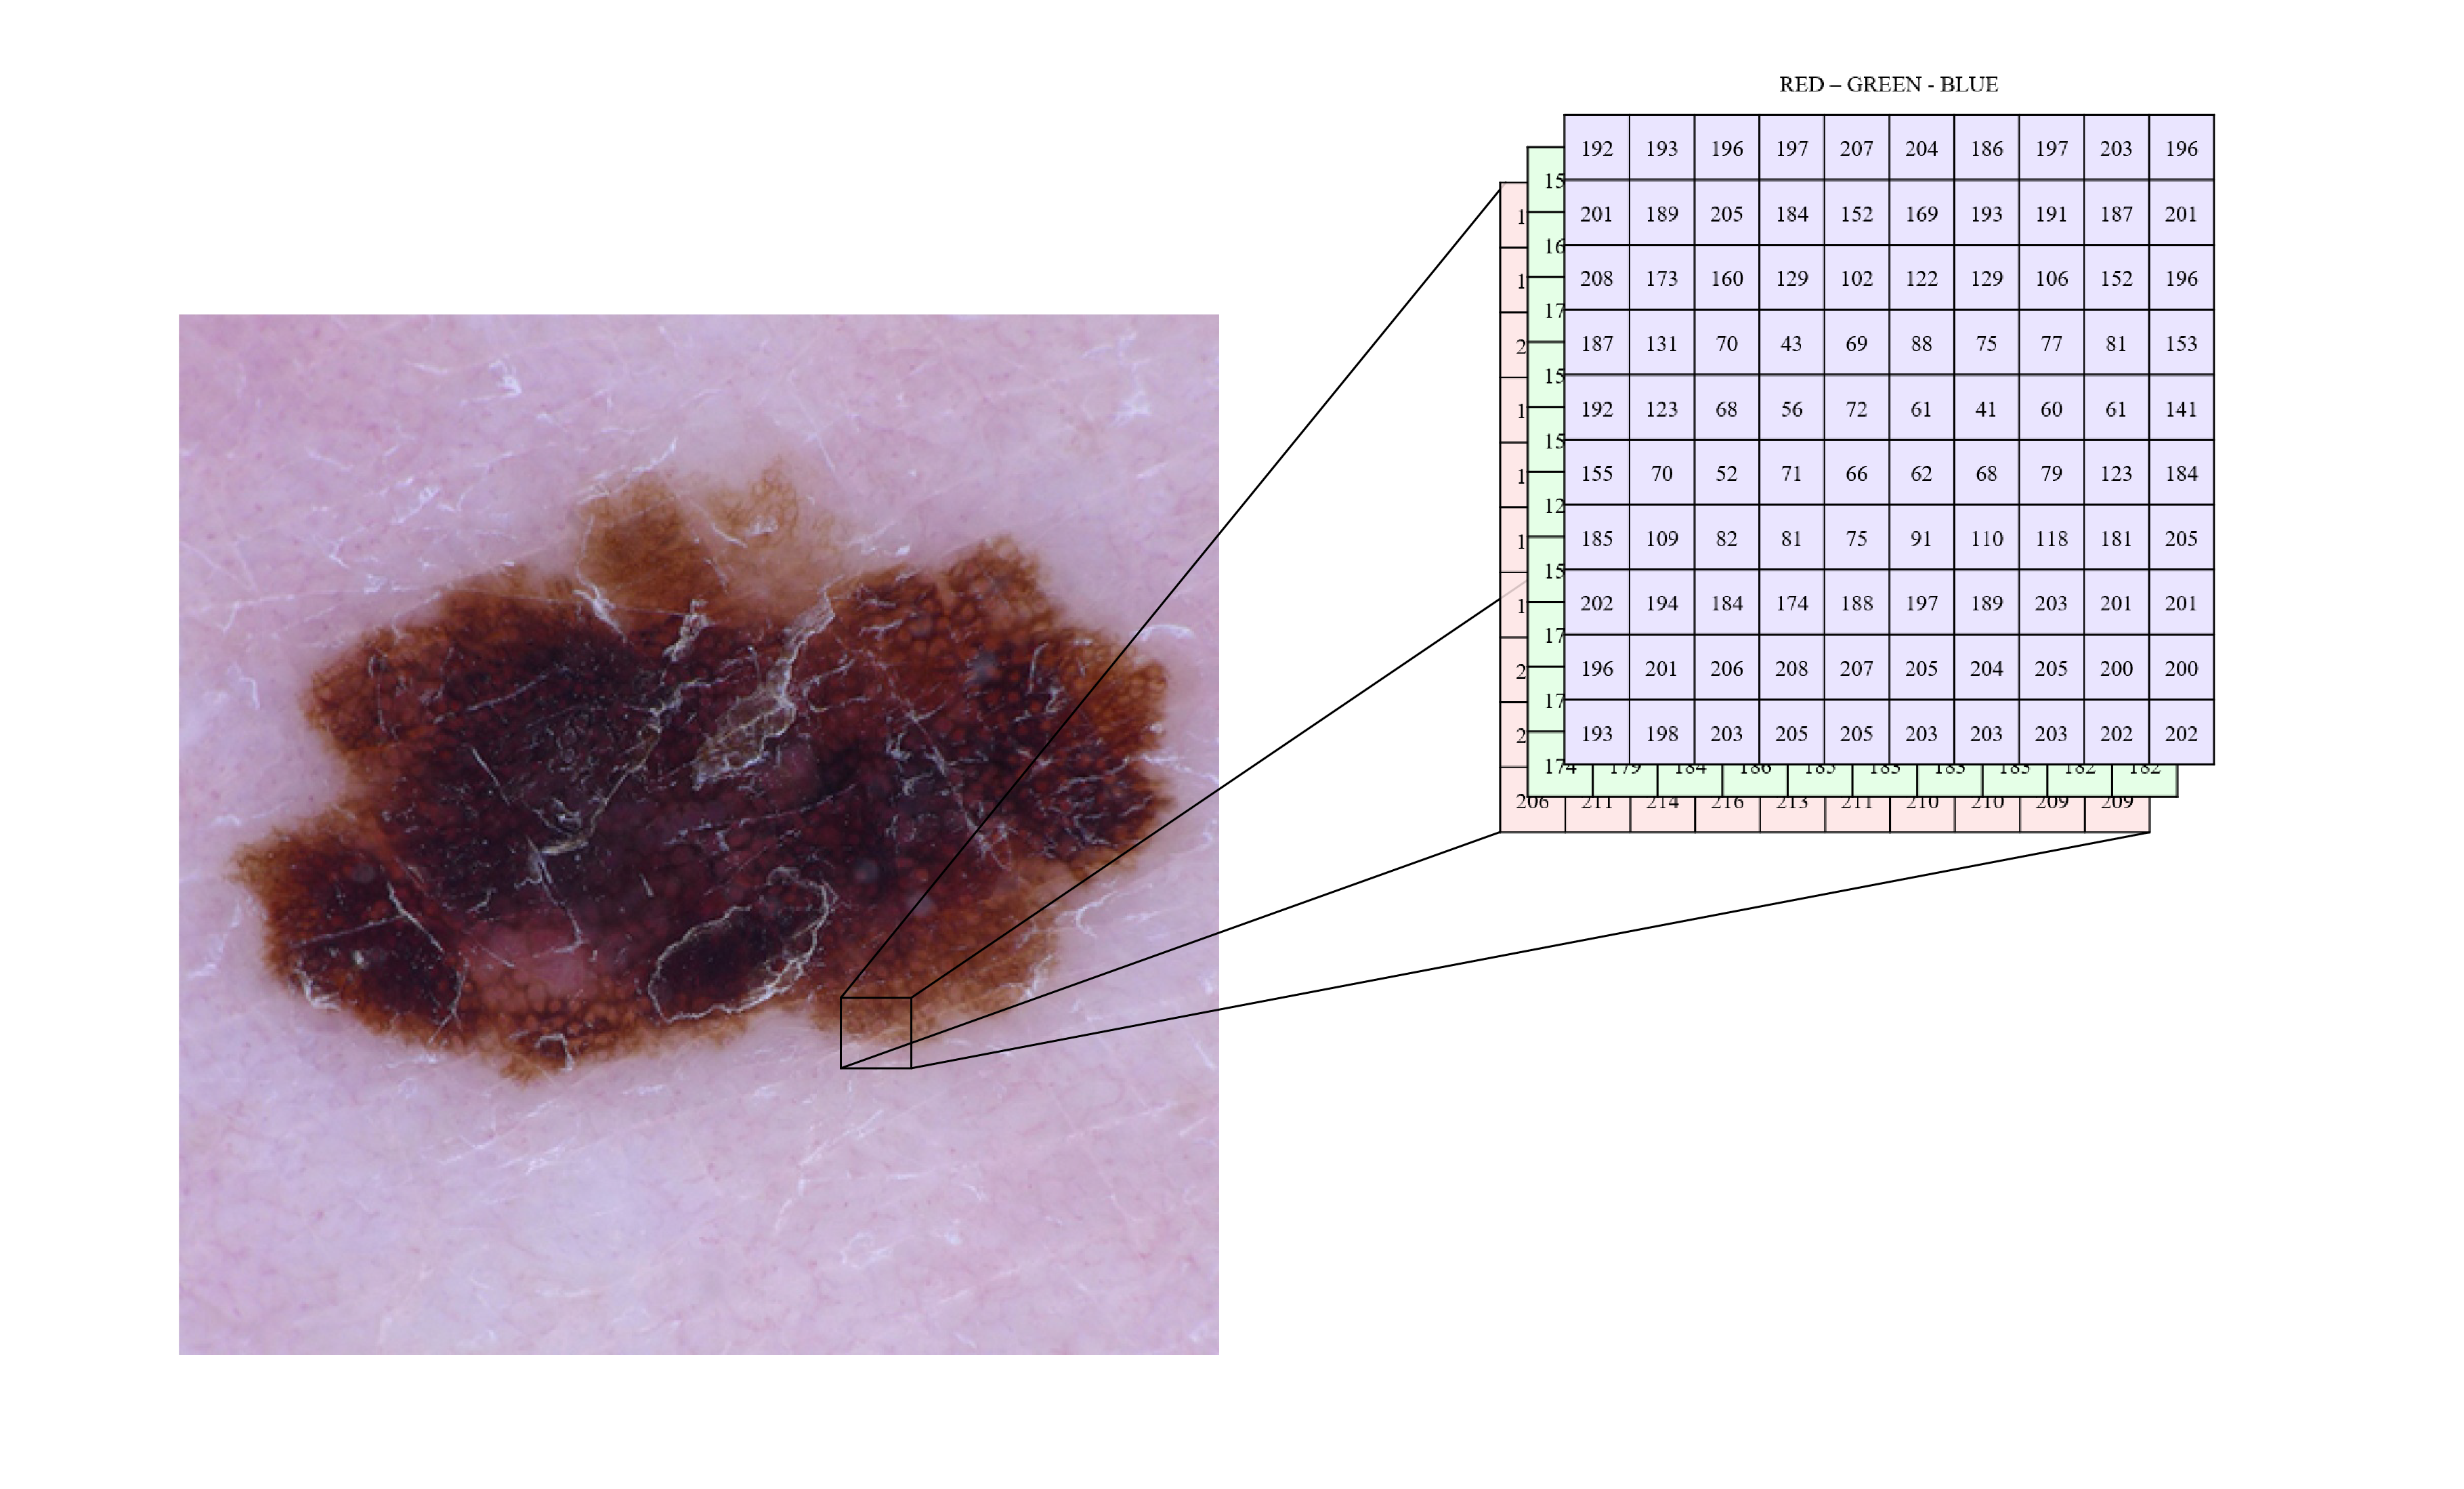
\includegraphics[width=8cm]{../img/Citra Warna - Latex.png}
            \caption{Citra warna beserta nilai pikselnya}
            \label{fig:color}
            Sumber: \citep{Kusumanto2011}
        \end{center}
    \end{figure}

    \subsection{Citra Skala Abu-Abu}
    Citra skala abu-abu merupakan citra yang memiliki satu kanal warna, yaitu menunjukkan intensitas derajat keabuan itu sendiri. Pada umumnya, nilai piksel yang dimiliki citra skala abu-abu berkisar antara 0 sampai 255 \citep{Kusumanto2011}. Gambar \ref{fig:grayscale} merupakan salah satu contoh citra skala abu-abu.

    \begin{figure}[H]
        \begin{center}
            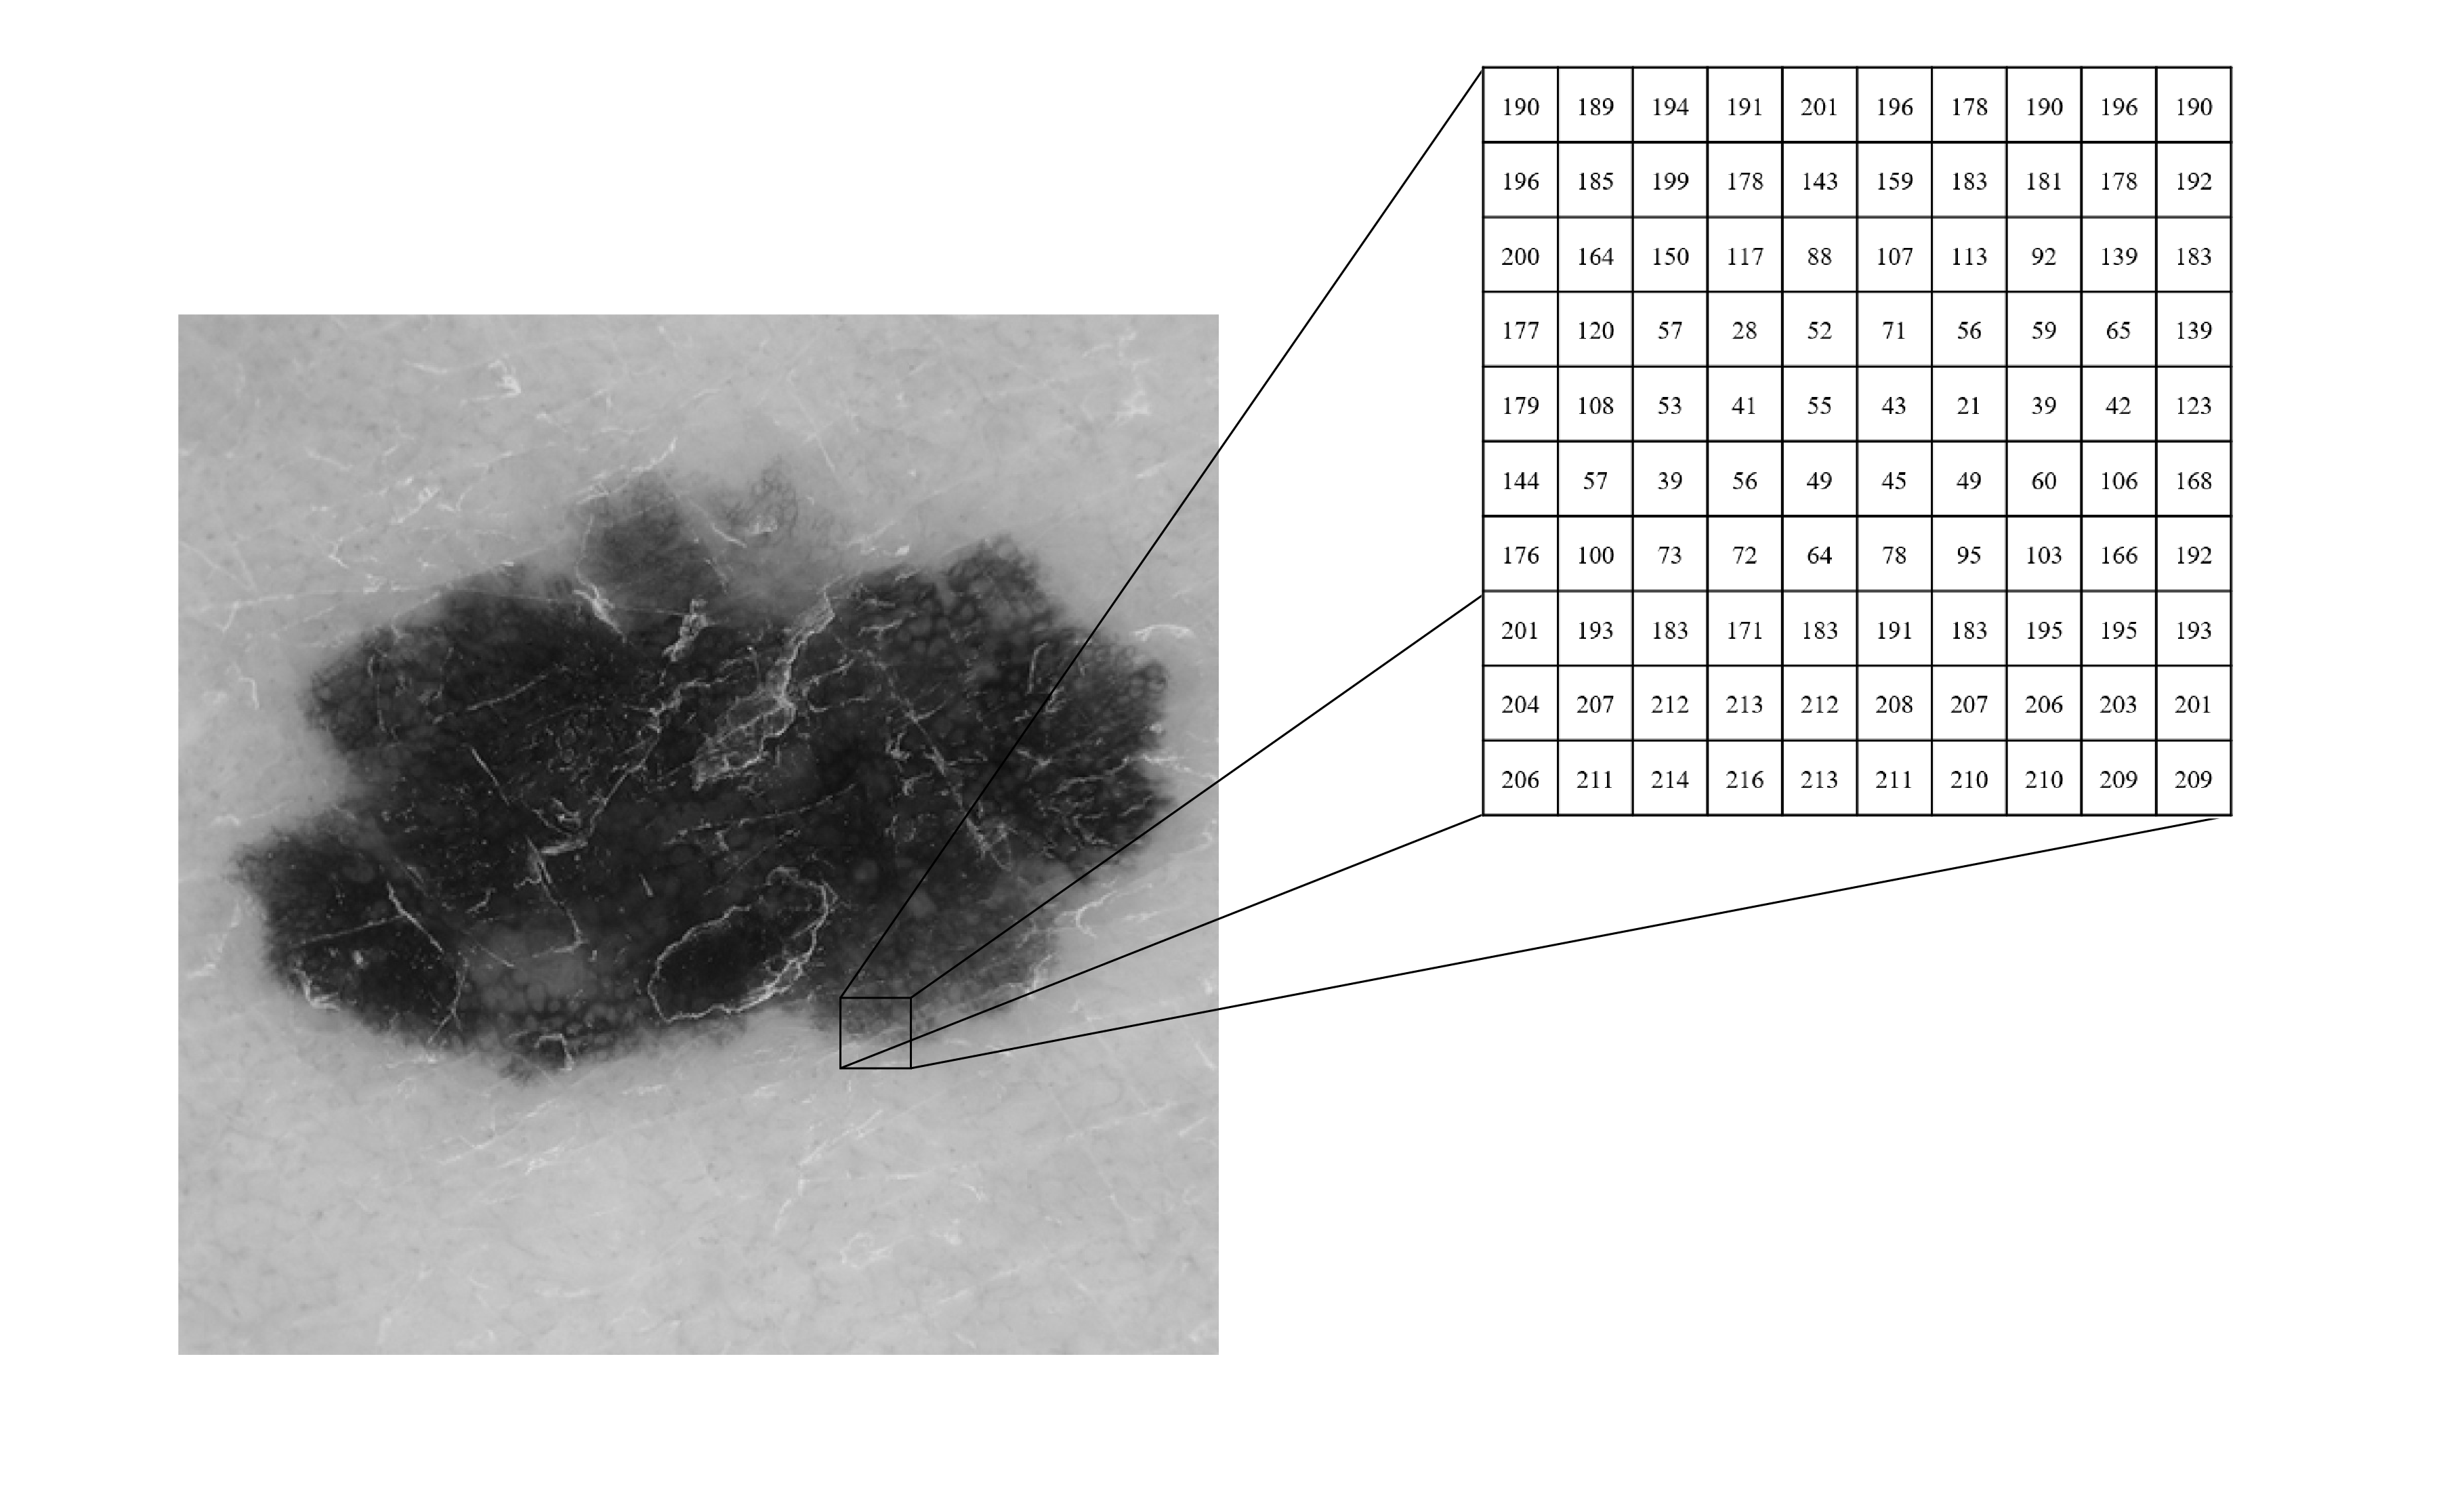
\includegraphics[width=8cm]{../img/Citra Grayscale - Latex.png}
            \caption{Citra \textit{grayscale} beserta nilai pikselnya}
            \label{fig:grayscale}
            Sumber: \citep{Kusumanto2011}
        \end{center}
    \end{figure}

    \subsection{Citra Biner}
    Citra biner merupakan citra yang hanya memiliki dua nilai, yaitu $0$ atau $1$. Citra ini termasuk citra yang paling sederhana karena nilai $0$ pada suatu piksel citra biner menggambarkan warna hitam sedangkan nilai $1$ menggambarkan warna putih \citep{Kusumanto2011}. Contoh citra biner seperti terlihat pada Gambar \ref{fig:binary}.

    \begin{figure}[H]
        \begin{center}
            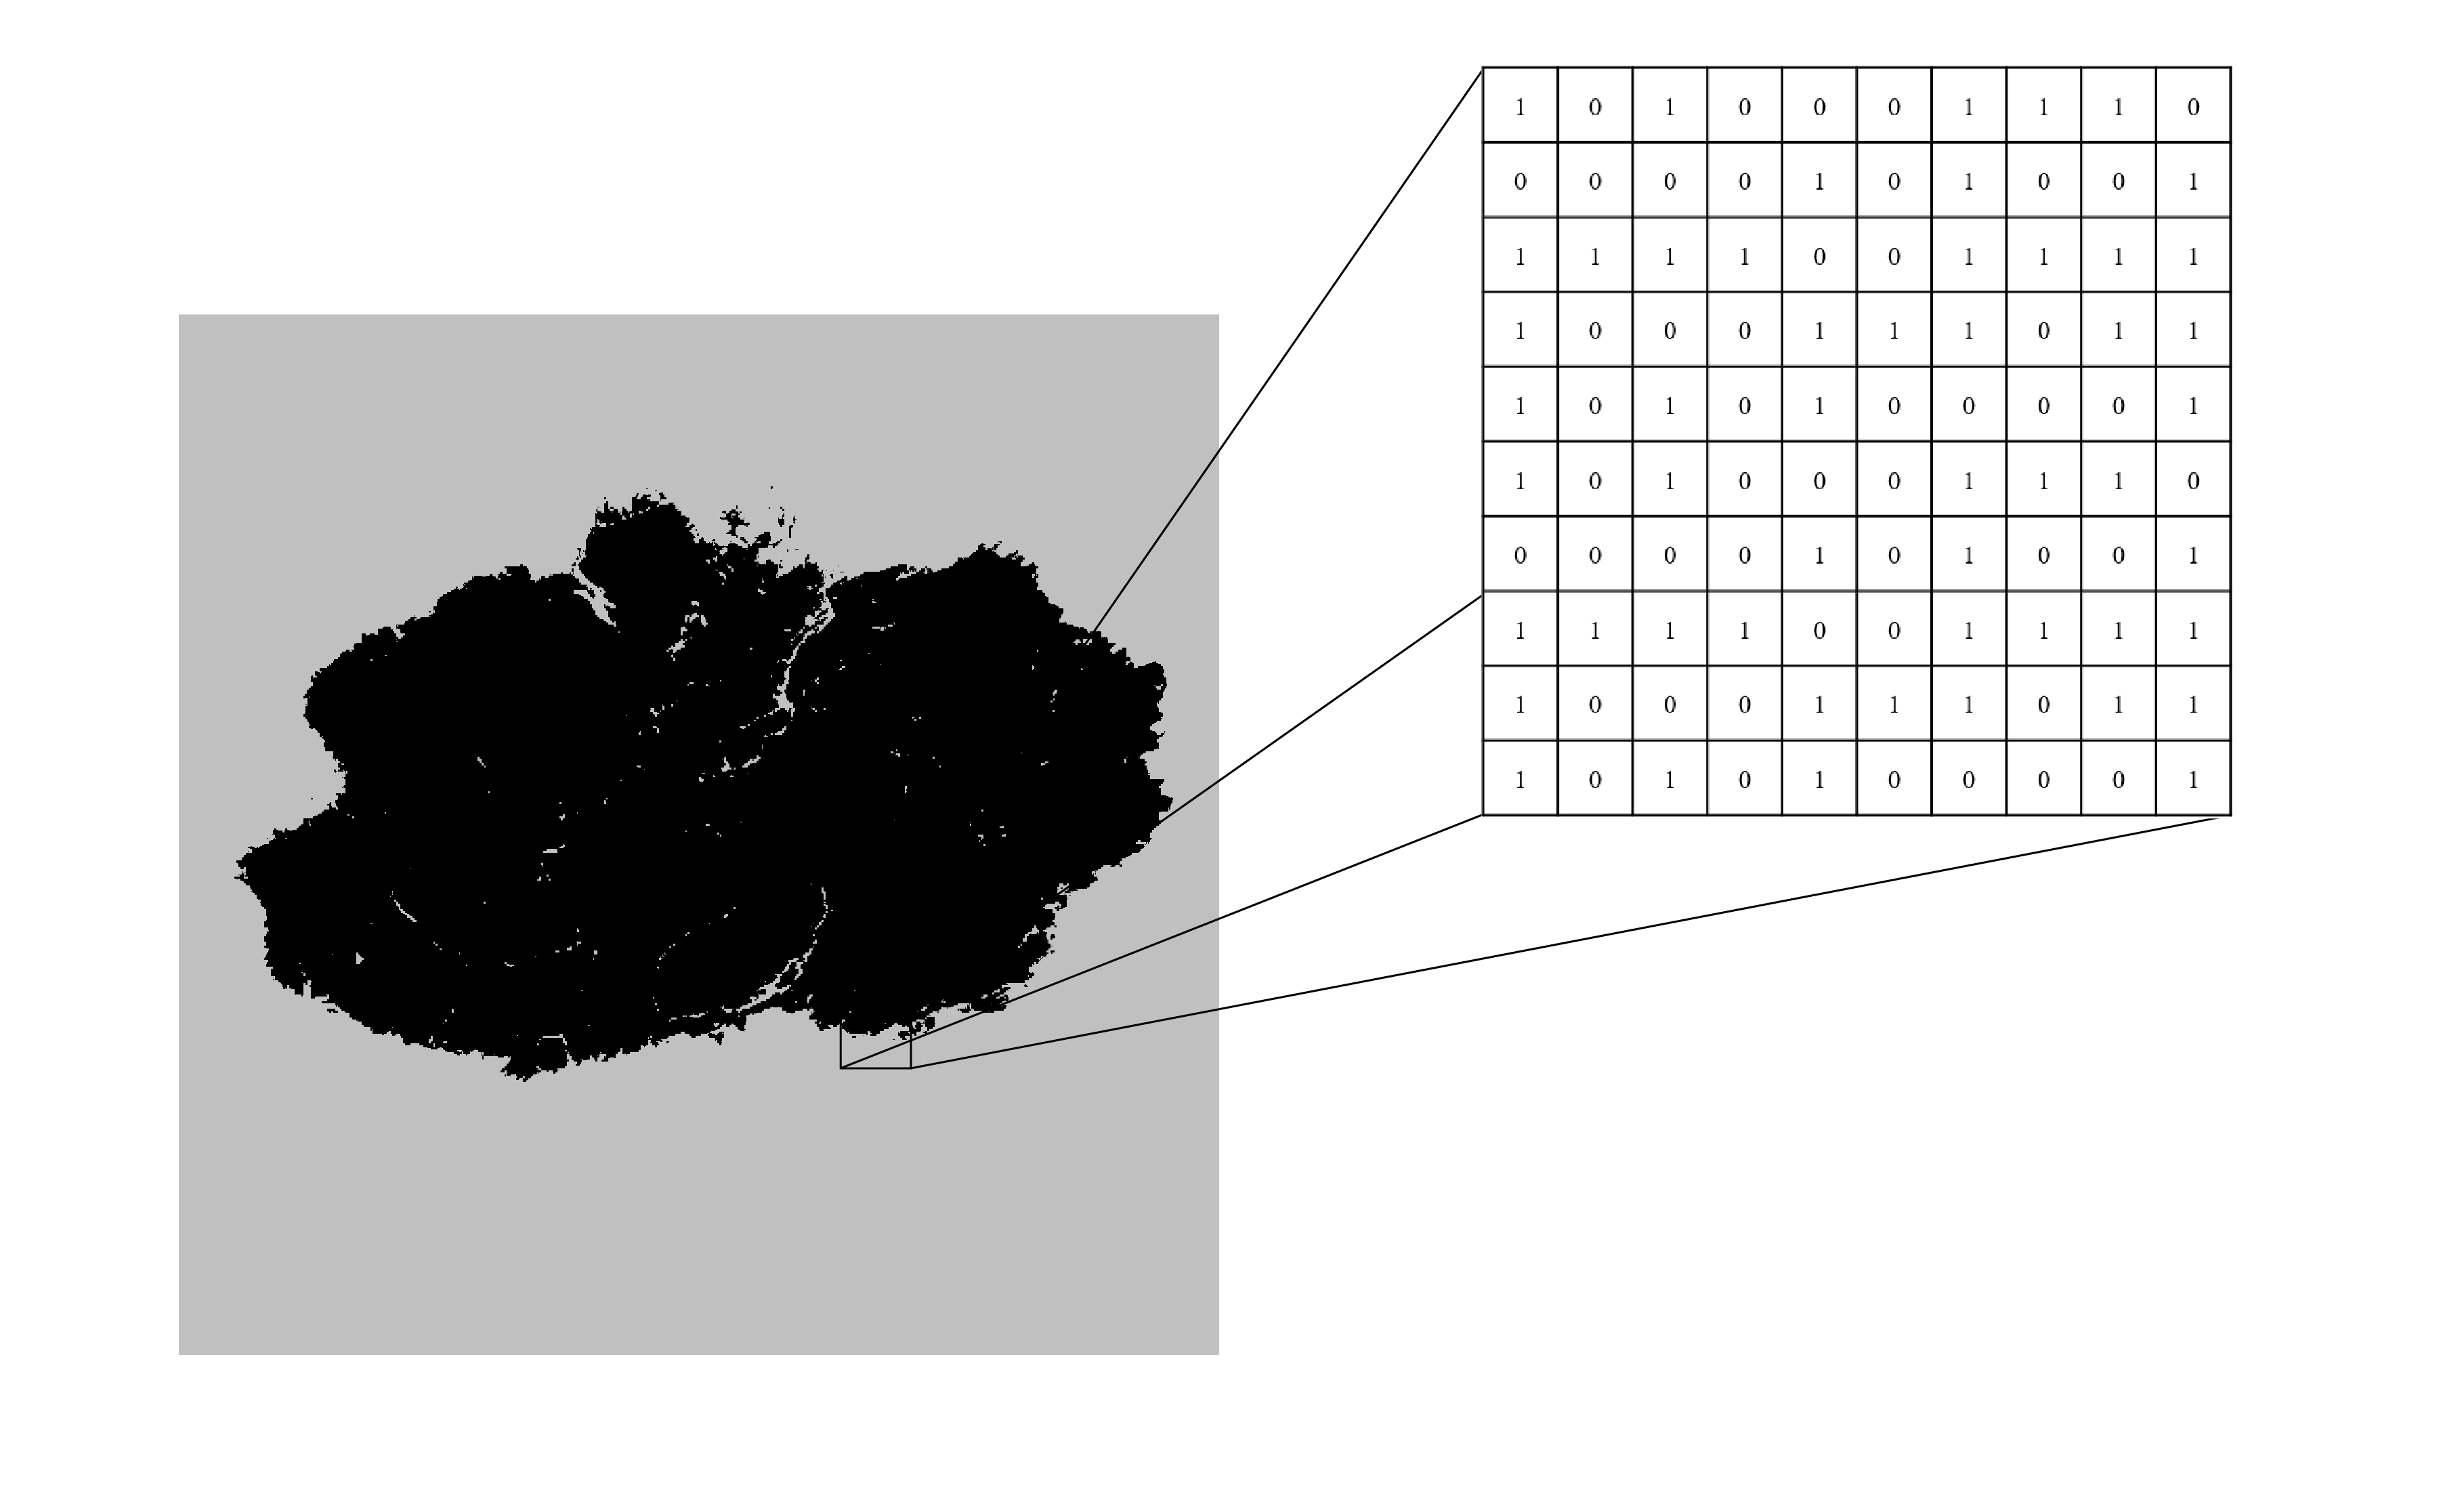
\includegraphics[width=8cm]{../img/Citra Biner - Latex.png}
            \caption{Citra biner beserta nilai pikselnya}
            \label{fig:binary}
            Sumber: \citep{Kusumanto2011}
        \end{center}
    \end{figure}

    % TODO: kurang jelas
    \subsection{Citra Dermoskopi}
    Dermoskopi menuju pada istilah dalam pemeriksaan kulit menggunakan mikroskop. Teknik ini merupakan teknik pencitraan kulit beresolusi tinggi yang memungkinkan visualisasi struktur kulit tanpa terhalang oleh pantulan permukaan kulit. Hal ini bertujuan untuk mengamati kulit dengan lebih detil dan mempermudah diagnosis kanker kulit. Sehingga, hasil dari teknik pencitraan kulit menggunakan mikroskop ini disebut sebagai citra dermoskopi \citep{Celebi2019}. Contoh citra dermoskopi seperti terlihat pada Gambar \ref{fig:dermoscopy}.

    \begin{figure}[H]
        \begin{center}
            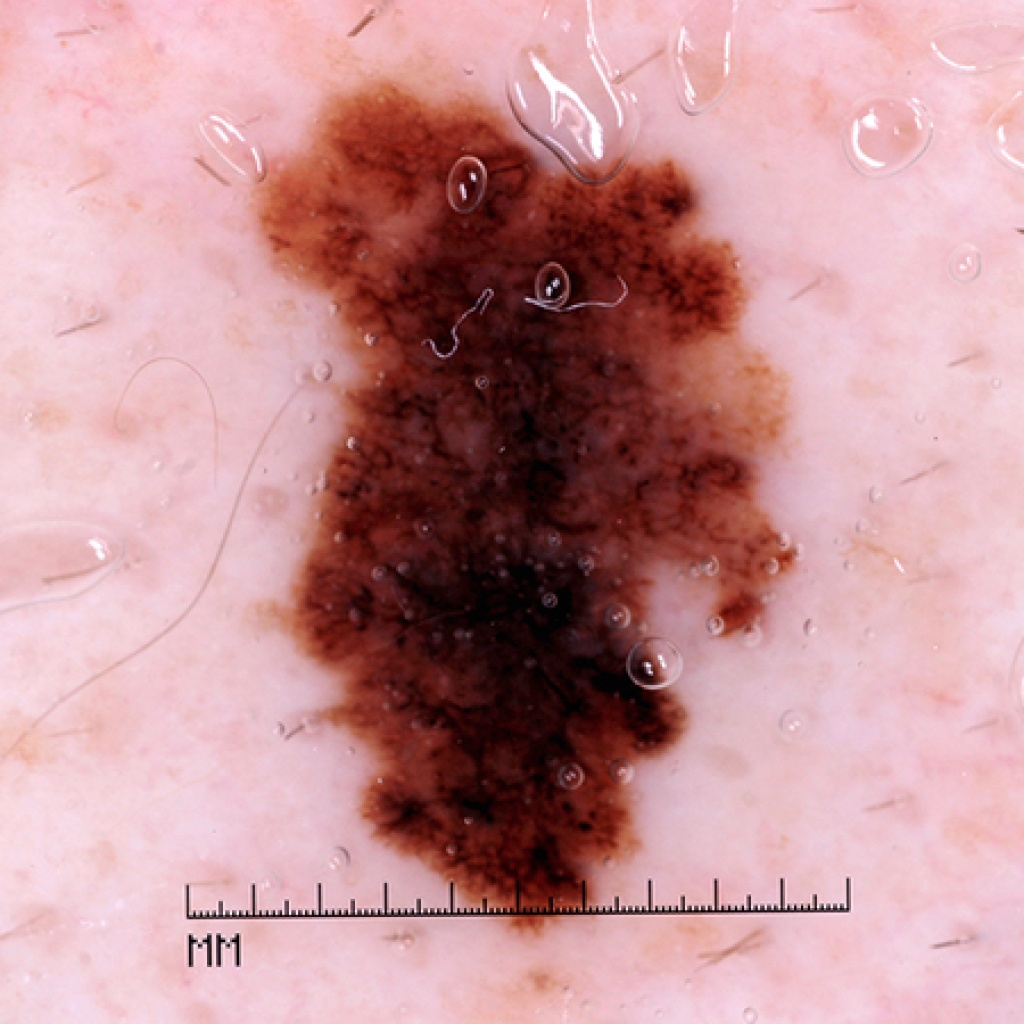
\includegraphics[width=4cm]{../img/Dermoscopy - Latex.jpg}
            \caption{Citra \textit{dermoscopy} yang mengandung kanker kulit \textit{melanoma}}
            \label{fig:dermoscopy}
            Sumber: \citep{Nersisson2021a}
        \end{center}
    \end{figure}

\section{\textit{Resize}}
\textit{Resize} atau penskalaan gambar merupakan proses rekontruksi citra untuk mengubah ukuran sebuah citra \citep{Morsy2018}. Pengubahan ukuran citra biasanya terjadi untuk menyesuaikan ukuran citra dan mengurangi waktu komputasi \citep{AhmedThaajwer2020a,Umamaheswari2018}. Penelitian ini menggunakan Interpolasi Bilinier untuk melakukan \textit{resize}. Perhitungan untuk melakukan \textit{resize} seperti terlihat pada \ref{eq:resize} dimana $w_x = \frac{x-x_1}{x_2-x_1}$ dan $w_y = \frac{y-y_1}{y_2-y_1}$. Pada persamaan \ref{eq:resize} $x$ merupakan lebar, $y$ merupakan tinggi, $(y_1, x_1)$, $(y_1, x_2)$, $(y_2, x_1)$, $(y_2, x_2)$ merupakan koordinat nilai piksel, $A$, $B$, $C$, $D$ merupakan nilai piksel, dan $Z$ merupakan nilai interpolasi antara dua nilai interpolasi $X$ dan $Y$ \citep{Gribbon2004}. Contoh penskalaan gambar seperti terlihat pada Gambar \ref{fig:resize}.

\begin{align}
    X &= A(1-w_x)+BW_x\nonumber\\
    Y &= C(1-w_x)+DW_x\nonumber\\
    Z &= X(1-w_y)+YW_y\nonumber\\
    \label{eq:resize}
    &= A(1-w_x)(1-w_y) + Bw_x(1-w_y) + C(1-w_x)w_y + Dw_{x}w_{y}
\end{align}

\begin{figure}[H]
    \centering
    \begin{tabular}{cc}
        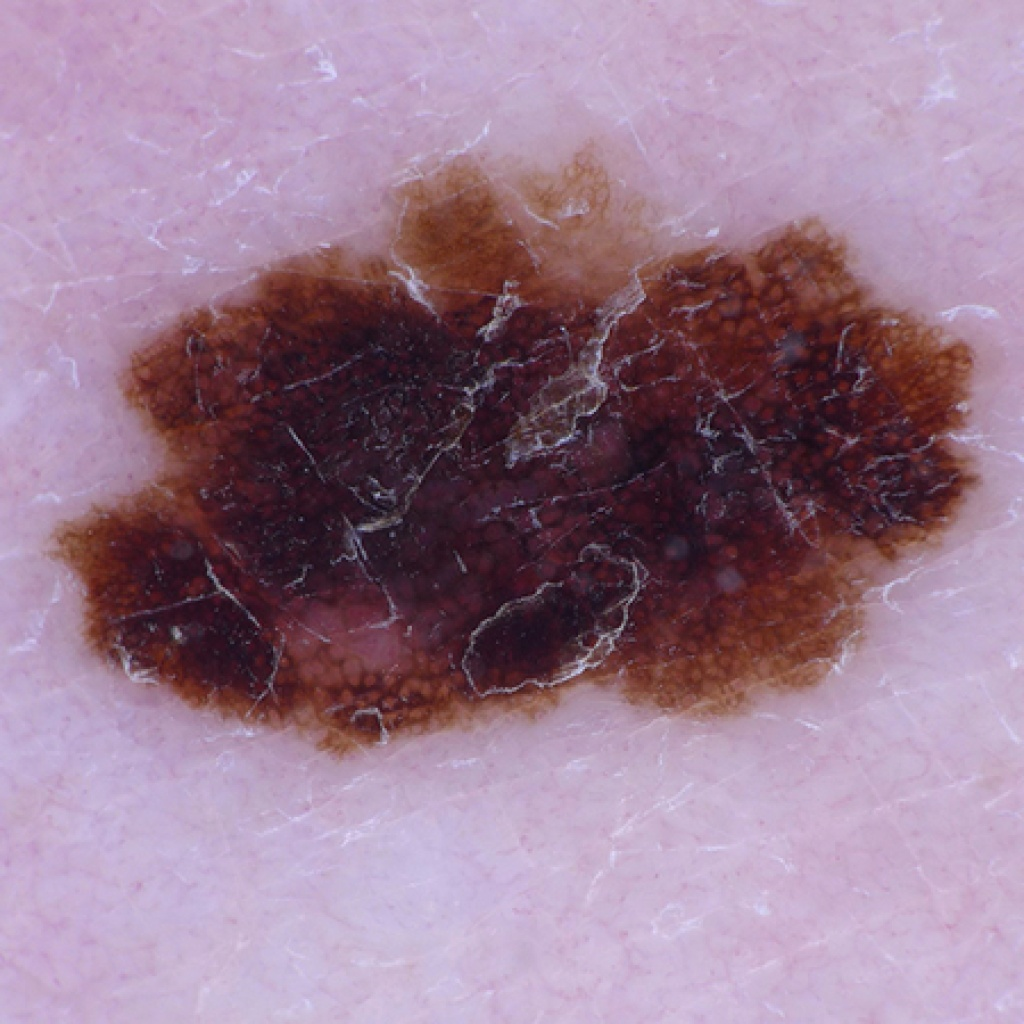
\includegraphics[width=4cm]{../img/Skin Cancer MEL - Latex.jpg}
        &
        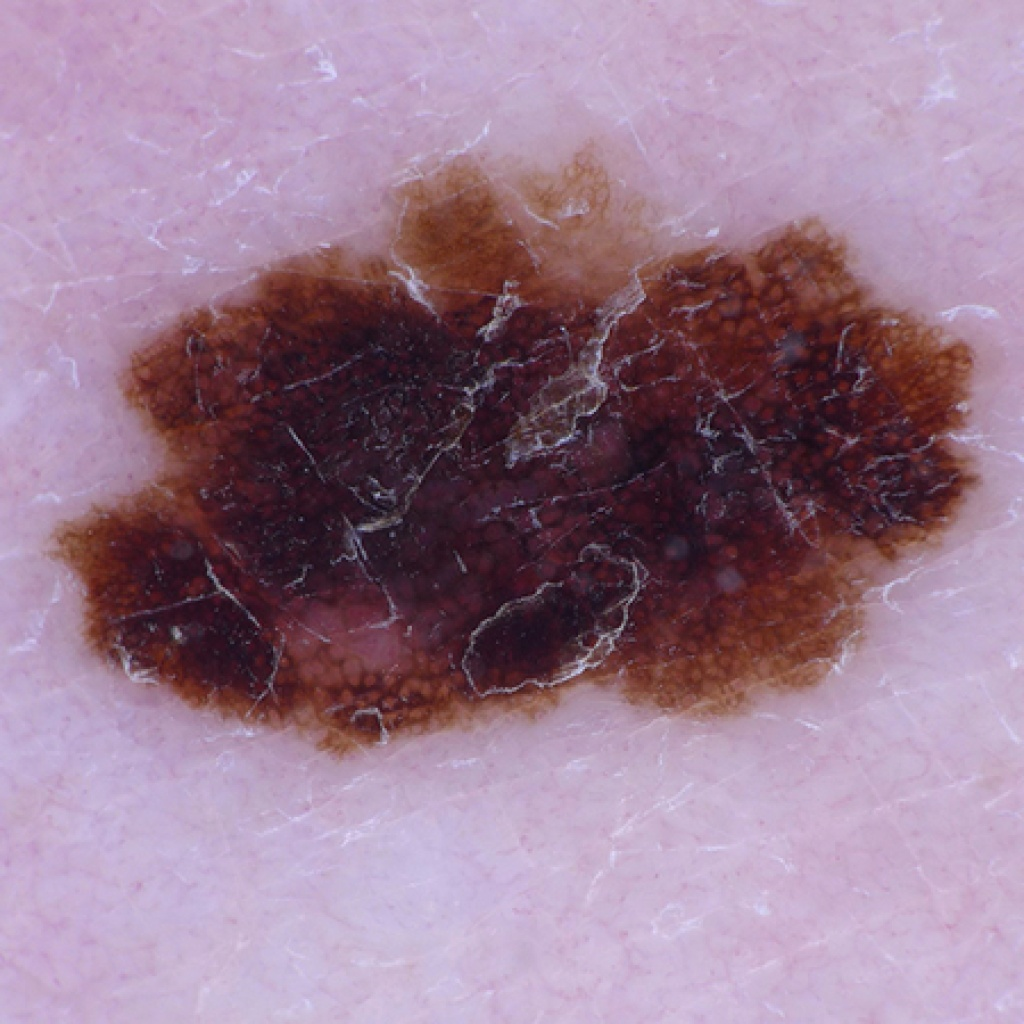
\includegraphics[width=2cm]{../img/Skin Cancer MEL - Latex.jpg}\\
        (a) &(b)\\
    \end{tabular}
    \caption{(a) Citra sebelum diubah berukuran $500\times 500$ piksel (b) Citra setelah diubah berukuran $200\times 200$ piksel}
    \label{fig:resize}
    Sumber: \citep{Morsy2018}
\end{figure}

\section{Deteksi Objek}
Deteksi objek merupakan salah satu proses penting dalam \textit{computer vision} dengan mendeteksi sebuah objek pada sebuah citra dengan kelas tertentu, misalnya mobil, manusia, hewan secara spesifik, atau yang lainnya. Sebagai salah satu bagian penting dalam \textit{computer vision}, deteksi objek merupakan dasar dari beberapa tugas \textit{computer vision} seperti melacak objek, segmentasi objek, dan mengambil teks dalam gambar \citep{Zou2019}. Contoh deteksi objek seperti terlihat pada Gambar \ref{fig:obj-det}.

\begin{figure}[H]
    \begin{center}
        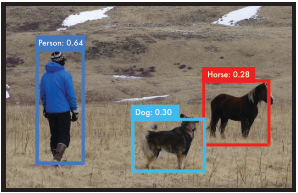
\includegraphics[width=7cm]{../img/Object Detection - Latex.png}
        \caption{YOLO dapat mendeteksi objek manusia, anjing, kuda}
        \label{fig:obj-det}
        Sumber: \citep{Redmon2016a}
    \end{center}
\end{figure}

\section{\textit{Convolutional Neural Networks} (CNN)}
CNN merupakan salah satu bagian dari deep learning dan pengembangan dari \textit{Multi Layer Perceptron} (MLP). CNN merupakan algoritma yang mirip dengan \textit{Artificial Neural Network} (ANN). Bahkan karena kemiripannya, strategi pengembangan ANN dapat diterapkan pada CNN. Data masukan pada CNN berupa matriks dari citra sehingga menghasilkan keluaran berupa skor atau bobot tertentu. Layer terakhir pada sebuah CNN mengandung loss function yang diasosiasikan dengan kelas tertentu. Pada umumnya, perbedaan ANN dan CNN terletak pada CNN yang lebih mengutamakan pengenalan pola pada sebuah citra. Hal ini dapat mengeluarkan fitur spesifik pada sebuah citra sehingga diolah pada arsitektur CNN.

Berdasarkan kemampuan CNN yang dapat mengolah data citra, neuron pada CNN terdiri atas neuron tiga dimensi. Neuron tersebut mengandung dimensi spasial dari data masukan, yaitu \textit{height}, \textit{width}, dan \textit{depth}. \textit{Depth} tidak mengacu pada jumlah layer pada jaringan, akan tetapi mengacu pada dimensi ketiga dari \textit{activation volume}. Neuron pada setiap layer hanya terkoneksi terhadap layer yang mendahuluinya. CNN terdiri dari tiga jenis layer, yaitu \textit{convolutional layer}, \textit{pooling layer}, dan \textit{fully-connected layers}. Arsitektur dasar pada CNN seperti terlihat pada Gambar \ref{fig:cnn}.

\begin{figure}[H]
    \begin{center}
        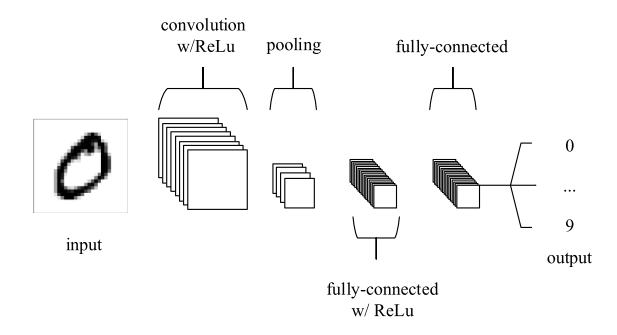
\includegraphics[width=12cm]{../img/CNN Basic - Latex.png}
        \caption{Arsitektur dasar dari CNN}
        \label{fig:cnn}
        Sumber: \citep{OShea2015}
    \end{center}
\end{figure}

\section{\textit{You Only Look Once version 7} (YOLO-v7)}
YOLO merupakan algoritma deteksi objek berdasarkan \textit{Fully Connected Neural Network} (FCNN). Algoritma ini dapat digunakan untuk mendeteksi objek secara \textit{real time}. Algoritma ini bekerja dengan membagi citra ke dalam beberapa kisi. Setiap kisi pada YOLO memiliki kemampuan untuk memprediksi objek dan \textit{bounding box}. \textit{Bounding box} merupakan kotak pembatas yang menandakan di dalamnya terdapat objek tertentu. Objek tersebut kemudian diklasifikasikan ke dalam kelas tertentu dengan memilih batas kotak yang memiliki nilai IoU paling tinggi. Secara umum, terdapat tiga komponen utama pada YOLO, yaitu \textit{backbone}, \textit{neck}, dan \textit{head}. \textit{Backbone} melakukan \textit{feature learning} kemudian diteruskan ke \textit{neck}. Bagian \textit{neck} mengumpulkan \textit{feature map} yang dipelajari dari \textit{backbone}. Pada akhirnya, \textit{head} memprediksi \textit{bounding box} dan probabilitas kelas yang ada di dalam \textit{bounding box}. YOLO merupakan metode yang populer dalam bidang \textit{computer vision} dan memunculkan banyak versi. Penelitian ini menggunakan YOLO-v7 dengan arsitektur seperti terlihat pada gambar \ref{fig:yolov7-archi}.
\begin{figure}[H]
    \begin{center}
        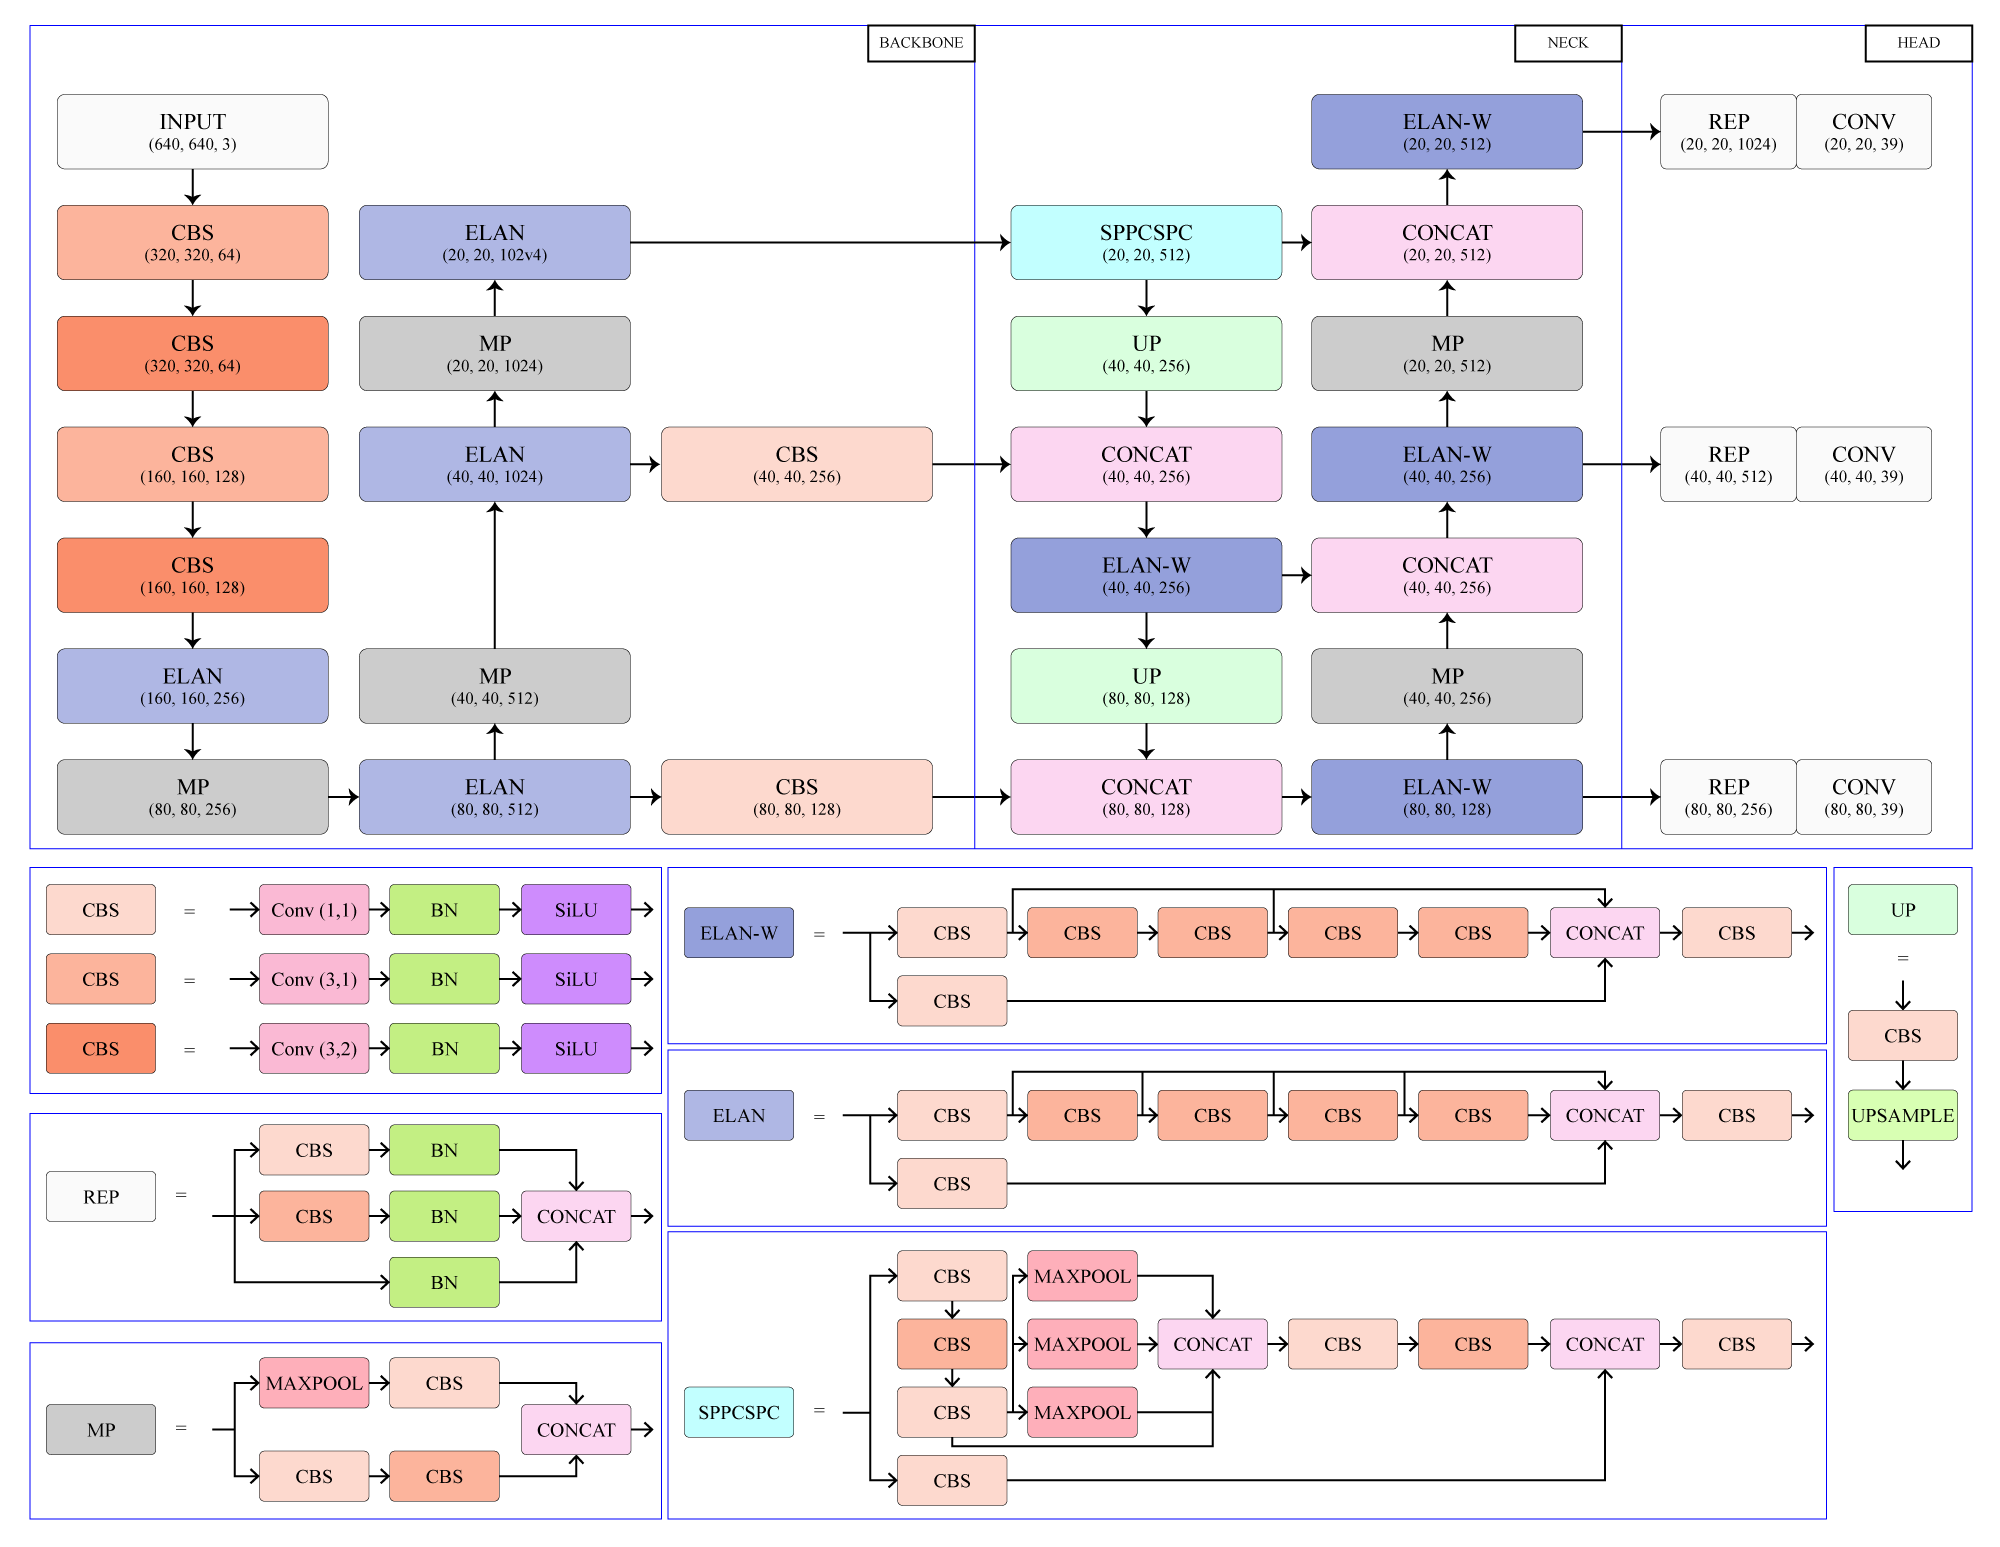
\includegraphics[width=13cm]{../img/YOLO-v7-Architecture.png}
        \caption{Arsitektur YOLO-v7}
        \label{fig:yolov7-archi}
        Sumber: \citep{Wang2022}
    \end{center}
\end{figure}

    \subsection{\textit{Convolutional Layer}}
    \textit{Convolutional Layer} merupakan layer utama dari CNN karena pada layer ini citra diolah dan dipelajari oleh CNN. \textit{Convolutional layer} menerapkan operasi konvolusi dengan tujuan mendapatkan fitur-fitur yang ada pada citra, seperti \textit{edge}, \textit{color}, \textit{shape}, dan fitur lainnya. Operasi konvolusi terjadi antara matriks dari data masukan, yaitu citra dan matriks kernel. Kernel mengubah nilai pada citra masukan sesuai dengan nilai pada kernel. Kernel memproses citra masukan dengan cara bergeser sebanyak \textit{stride} yang ditentukan. Hasil keluaran dari \textit{convolutional layer} berupa \textit{feature map} yang didapatkan dari sebuah citra masukan. Perhitungan untuk mendapatkan \textit{feature map} seperti terlihat pada persamaan \ref{eq:conv-layer} dimana $z$ merupakan keluaran dari layer $l$, $h$ merupakan citra masukan, $W$ merupakan kernel, dan $b$ merupakan bias. Gambar \ref{fig:conv} menunjukkan representasi dari \textit{convolutional layer} \citep{OShea2015}.

    \begin{align}
        \label{eq:conv-layer}
        z^l &= h^{l-1}\ast W^l + b^l
    \end{align}

    \begin{figure}[H]
        \begin{center}
            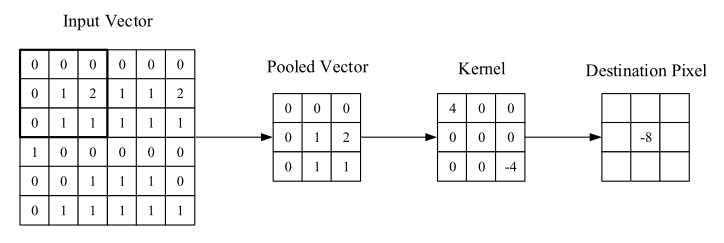
\includegraphics[width=12cm]{../img/CNN Convolutional Layer - Latex.png}
            \caption{Cara kerja kernel pada \textit{convolutional layer}}
            \label{fig:conv}
            Sumber: \citep{OShea2015}
        \end{center}
    \end{figure}

    \subsection{\textit{Pooling Layer}}
    \textit{Pooling layer} merupakan layer yang memproses \textit{feature map} dari \textit{convolutional layer}. Layer ini berfungsi untuk mengurangi volume pada setiap tumpukan \textit{feature map} tanpa menghilangkan informasi yang dibutuhkan. Terdapat beberapa jenis \textit{pooling layer} seperti, \textit{max pooling} dan \textit{average pooling}. YOLO-v7 menggunakan \textit{max pooling} dalam arsitekturnya. \textit{Max pooling} mengambil nilai tertinggi pada \textit{feature map} berdasarkan ukuran kernel. Perhitungan \textit{max pooling} seperti terlihat pada persamaan \ref{eq:max-pool} dimana $i=0, \cdots, n;j=0, \cdots, n$. Hasil aktivasi \textit{layer} $l$ adalah $h^{l}_{xy}$ dengan $xy$ yang merepresentasikan baris dan kolom. Proses \textit{max pooling} seperti terlihat pada Gambar \ref{fig:max-pool}.

    \begin{align}
        \label{eq:max-pool}
        h^{l}_{xy} &= max_{ij}(h^{l-1}_{(x+i)(y+j)})
    \end{align}

    \begin{figure}[H]
        \centering
        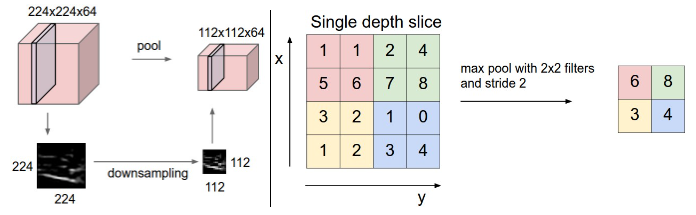
\includegraphics[width=10cm]{../img/Max Pooling - Latex.png}
        \caption{Cara kerja \textit{max pooling} yang digunakan pada YOLO-v7}
        \label{fig:max-pool}
        Sumber: \citep{Yani2019}
    \end{figure}

    \subsection{\textit{Upsample Layer}}
    \textit{Upsample layer} merupakan \textit{layer} yang dapat meningkatkan ukuran \textit{feature map}. \textit{Layer} ini mengembalikan ukuran seperti yang digunakan pada \textit{layer} sebelumnya. Rumus untuk mengimplementasikan \textit{upsample layer} seperti terlihat pada persamaan \ref{eq:upsample} dimana $R$ dan $C$ merupakan tinggi dan lebar data asli sedangkan $R'$ dan $C'$ merupakan tinggi dan lebar data setelah \textit{upsampling}.

    \begin{align}
        \label{eq:upsample}
        S_r &= \frac{R-1}{R'}\nonumber\\
        S_c &= \frac{C-1}{C'}
    \end{align}

    \subsection{\textit{Batch Normalization} (BN)}
    Pada umumnya, hampir setiap metode \textit{deep learning} mengimplementasikan BN. BN merupakan teknik yang dapat mempercepat proses pelatihan model dan membuat proses pelatihan lebih stabil. Teknik ini melakukan normalisasi vektor pada \textit{hidden layers} menggunakan rata-rata dan varian. BN dapat dilakukan sebelum atau sesudah menjalankan fungsi non-linier. Pada setiap \textit{hidden layer}, BN mengubah nilai pada hidden layer menggunakan persamaan \ref{eq:bn-1}-\ref{eq:bn-4}.

    \begin{align}
        \label{eq:bn-1}
        \mu &= \frac{1}{n} \sum_i Z^{(i)}\\
        \label{eq:bn-2}
        \sigma^2 &= \frac{1}{n} \sum_i (Z^{(i)}-\mu)^2\\
        \label{eq:bn-3}
        Z^{(i)}_{norm} &= \frac{Z^{(i)}-\mu}{\sqrt{\sigma-\epsilon}}\\
        \label{eq:bn-4}
        \breve{Z} &= \gamma \ast Z^{(i)}_{norm}+\beta
    \end{align}

    Pertama, BN menghitung nilai rata-rata dan varian menggunakan persamaan \ref{eq:bn-1} dan \ref{eq:bn-2}. Kemudian dilakukan normalisasi menggunakan persamaan \ref{eq:bn-3} sehingga data keluaran berdistribusi normal dimana $\epsilon$ berupa konstanta untuk stabilitas numerik. Langkah terakhir menghitung keluaran $\breve{Z}$ dengan menerapkan transformasi linier terhadap $\gamma$ dan $\beta$ seperti persamaan \ref{eq:bn-4}.

    \subsection{\textit{Leaky Rectified Linear Unit} (Leaky ReLU)}
    ReLU merupakan fungsi aktivasi yang sering digunakan pada masalah \textit{computer vision} saat ini. ReLU memiliki tingkat konvergensi yang lebih baik daripada fungsi aktivasi sigmoid dan tanh. Hasil keluaran ReLU memiliki ambang batas $0$ sehingga jaringan lebih cepat karena memiliki perhitungan yang efisien. Akan tetapi, ReLU memiliki masalah \textit{Dying ReLU} dimana ReLU tidak berfungsi untuk semua data masukan karena bernilai kurang dari nol. Berawal dari hal ini, Leaky ReLU muncul dengan mengubah gradien ReLU sedikit ke kiri sehingga Leaky ReLU dapat menghasilkan beberapa nilai jika data masukan kurang dari nol. Rumus Leaky ReLU seperti terlihat pada persamaan \ref{eq:l-relu}. Grafik Leaky ReLU seperti terlihat pada gambar \ref{fig:l-relu} \citep{Xu2015}.

    \begin{align}
        \label{eq:l-relu}
        f(x) &= max(0.1x, x)
    \end{align}

    \begin{figure}[H]
        \begin{center}
            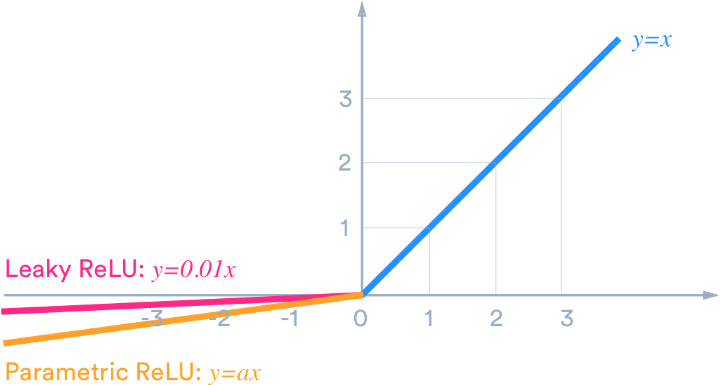
\includegraphics[width=8cm]{../img/Leaky ReLU - Latex.png}
            \caption{Grafik Leaky ReLU}
            \label{fig:l-relu}
            Sumber: \citep{Xu2015}
        \end{center}
    \end{figure}

    \subsection{\textit{Sigmoid-weighted Linear Unit} (SiLU)}
    SiLU merupakan salah satu fungsi aktivasi yang diusulkan untuk \textit{reinforcement learning}. Fungsi aktivasi SiLU dihitung dengan melakukan operasi perkalian antara fungsi sigmoid dengan data masukan. Rumus SiLU seperti terlihat pada persamaan \ref{eq:silu}. Grafik SiLU tidak menaik secara monoton seperti ReLU, akan tetapi sedikit melandai ke bawah dengan nilai minimum sekitar $-0.28$ untuk $z_k \approx -1.28$. Grafik SiLU seperti terlihat pada Gambar \ref{fig:silu}.

    \begin{align}
        \label{eq:silu}
        a_k(z_k) &= z_k\sigma (z_k)\nonumber\\
        &= z_k\frac{1}{1+e^{-(z_k)}}
    \end{align}

    \begin{figure}[H]
        \begin{center}
            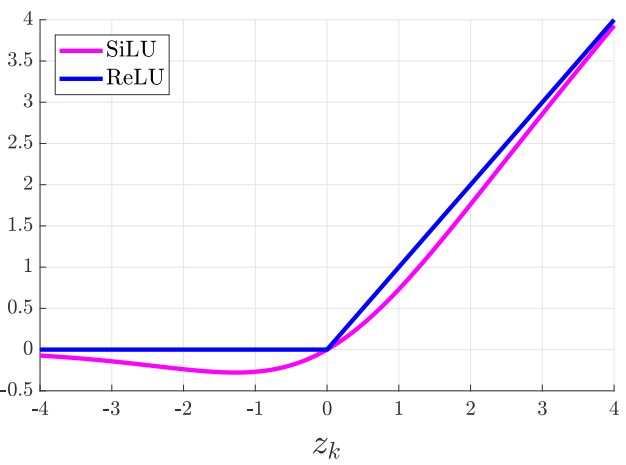
\includegraphics[width=8cm]{../img/SiLU - Latex.PNG}
            \caption{Perbandingan grafik SiLU dan ReLU}
            \label{fig:silu}
            Sumber: \citep{Elfwing2018}
        \end{center}
    \end{figure}

    \subsection{\textit{Efficient Layer Aggregation Networks} (ELAN)}
    ELAN merupakan jaringan yang melakukan proses agregasi fitur dan transfer fitur. Pada YOLO-v7, ELAN berada pada bagian \textit{backbone} sehingga ELAN bertugas untuk melakukan \textit{feature learning}. Modul ini memiliki struktur jaringan dan proses komputasi pemanfaatan parameter yang efisien sehingga jaringan dapat mempelajari fitur yang lebih beragam. ELAN memiliki dua cabang. Cabang pertama melakukan konvolusi $1\times 1$ untuk mengurangi \textit{depth}. Cabang kedua melakukan konvolusi $1\times 1$ kemudian melalui empat modul konvolusi $3\times 3$ yang berguna untuk \textit{feature learning}. Pada akhirnya, keempat fitur digabungkan untuk mendapatkan fitur akhir. Terdapat dua jenis ELAN, yaitu ELAN dan ELAN-W dimana perbedaan keduanya terdapat pada output yang diteruskan pada cabang kedua. Struktur jaringan ELAN dan ELAN-W seperti terlihat pada gambar \ref{fig:elan}.
    
    \begin{figure}[H]
        \centering
        \begin{tabular}{c}
            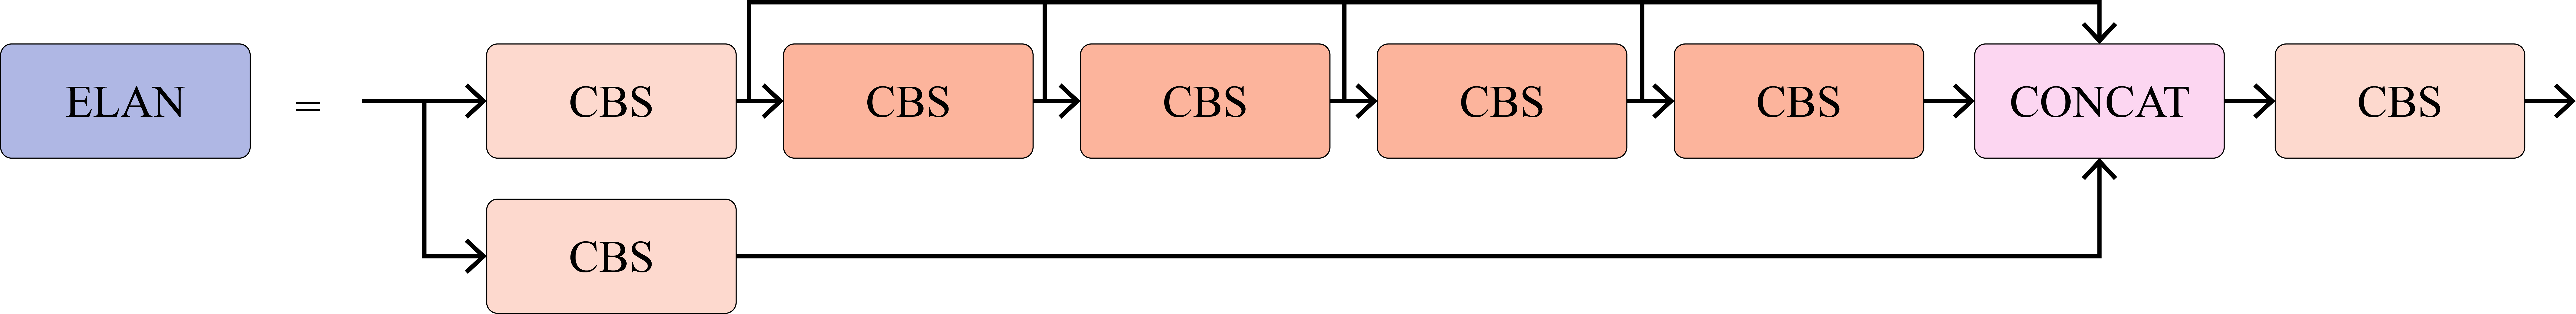
\includegraphics[width=13cm]{../img/ELAN.png}\\
            (a)\\
            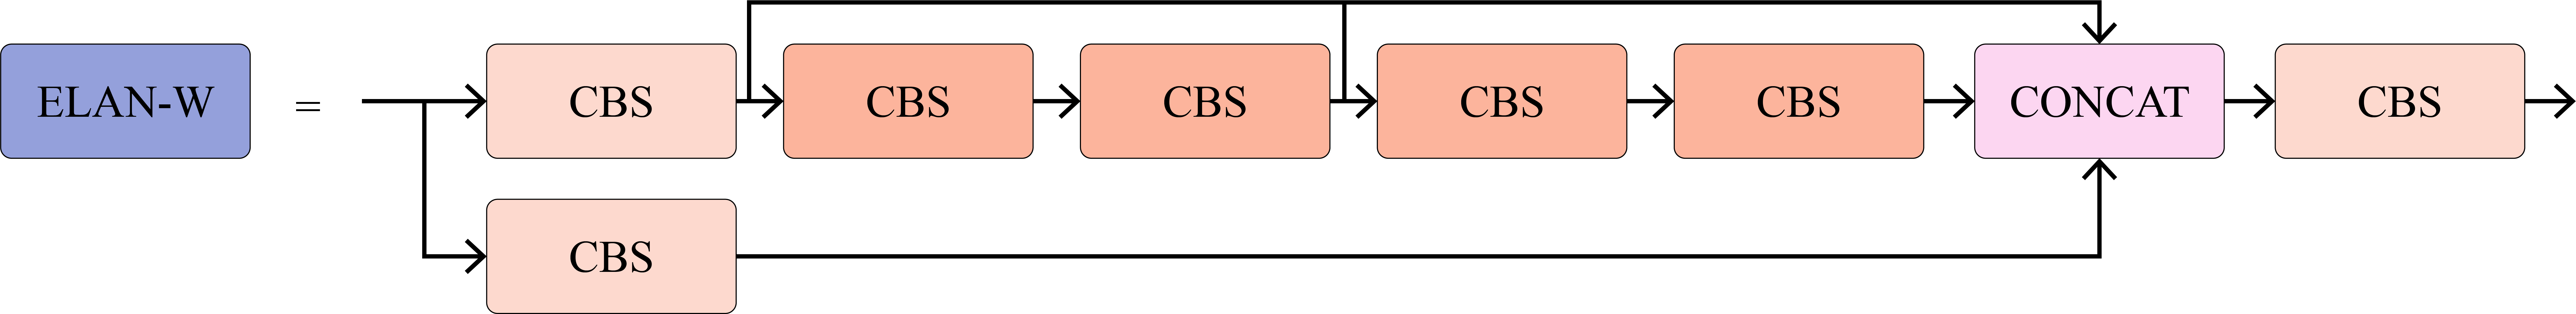
\includegraphics[width=13cm]{../img/ELAN-W.png}\\
            (b)\\
        \end{tabular}
        \caption{Struktur jaringan ELAN (a) ELAN; (b) ELAN-W}
        \label{fig:elan}
        Sumber: \citep{Wang2022}
    \end{figure}

    % TODO: Turunan dari activation function masukkan ke dalam BAB II

\section{\textit{Confusion Matrix}}
\textit{Confusion matrix} merupakan salah satu metrik yang dapat menggambarkan performa dari sebuah algoritma klasifikasi. Secara matematis, \textit{confusion matrix} berupa matrix $C_{ij}$ yang berisi nilai integer yang tidak negatif dengan $i=1\cdots n,j=1\cdots n$ dimana $n$ merupakan jumlah kelas pada permasalahan klasifikasi. Elemen $C_{ij}$ merupakan hasil klasifikasi selama proses pengujian model. Jika $i=j$ maka kelas $i$ terklasifikasi dengan benar pada kelas $j$. Sehingga dapat dikatakan elemen pada diagonal utama matriks merupakan semua kelas yang terklasifikasi dengan benar. Sedangkan elemen tidak nol lainnya menandakan kesalahan klasifikasi \citep{Susmaga2004}. Setiap elemen pada \textit{confusion matrix} termasuk ke dalam beberapa kategori berikut \citep{Shultz2017}:
\begin{enumerate}
    \item \textit{True Positive} (TP) menunjukkan ketepatan model dalam mengklasifikasikan kelas positif sebagai kelas positif.
    \item \textit{False Positive} (FP) menunjukkan ketepatan model dalam mengklasifikasikan kelas positif sebagai kelas negatif.
    \item \textit{True Negative} (TN) menunjukkan ketepatan model dalam mengklasifikasikan kelas negatif sebagai kelas negatif.
    \item \textit{False Negative} (FN) menunjukkan ketepatan model dalam mengklasifikasikan kelas negatif sebagai kelas positif.
\end{enumerate}

Sehingga \textit{confusion matrix} dapat digambarkan ke dalam sebuah tabel seperti terlihat pada Tabel \ref{tab:conf-mat}. Pada Tabel \ref{tab:conf-mat} terdapat $1\cdots n$ kelas. Baris dan kolom pada Tabel \ref{tab:conf-mat} berturut-turut merepresentasikan data aktual dan hasil klasifikasi.

\begin{table}[H]
    \caption{\textit{Confusion matrix}}
    \centering
    \begin{tabular}{|c|c|c|c|c|}
        \hline
        \           &$1$        &$2$        &$\cdots$   &$n$\\
        \hline
        $1$         &$C_{11}$   &$FN$       &$\cdots$   &$C_{1n}$\\
        \hline
        $2$         &$FP$       &$TP$       &$\cdots$   &$FP$\\
        \hline
        $\vdots$    &$\vdots$   &$\vdots$   &$\ddots$   &$\vdots$\\
        \hline
        $n$         &$C_{n1}$   &$FN$       &$\cdots$   &$C_{nn}$\\
        \hline
    \end{tabular}

    \label{tab:conf-mat}
    Sumber: \citep{Shultz2017}
\end{table}

\section{\textit{Intersection over Union} (IoU)}
IoU merupakan indikasi untuk mengetahui seberapa tepat prediksi kotak pembatas ke terhadap objek yang ada pada citra. Semakin tinggi nilai IoU menandakan semakin baik prediksi kotak pembatas oleh model deteksi objek. Kondisi IoU seperti terlihat pada Gambar \ref{fig:iou-cond} (a) dimana $(x_1, y_1)$ dan $(x_2, y_2)$ merupakan koordinat kotak pembatas data aktual sedangkan $(x_3, y_3)$ dan $(x_4, y_4)$ merupakan koordinat kotak pembatas hasil prediksi.

\begin{figure}[H]
    \centering
    \begin{tabular}{ccc}
        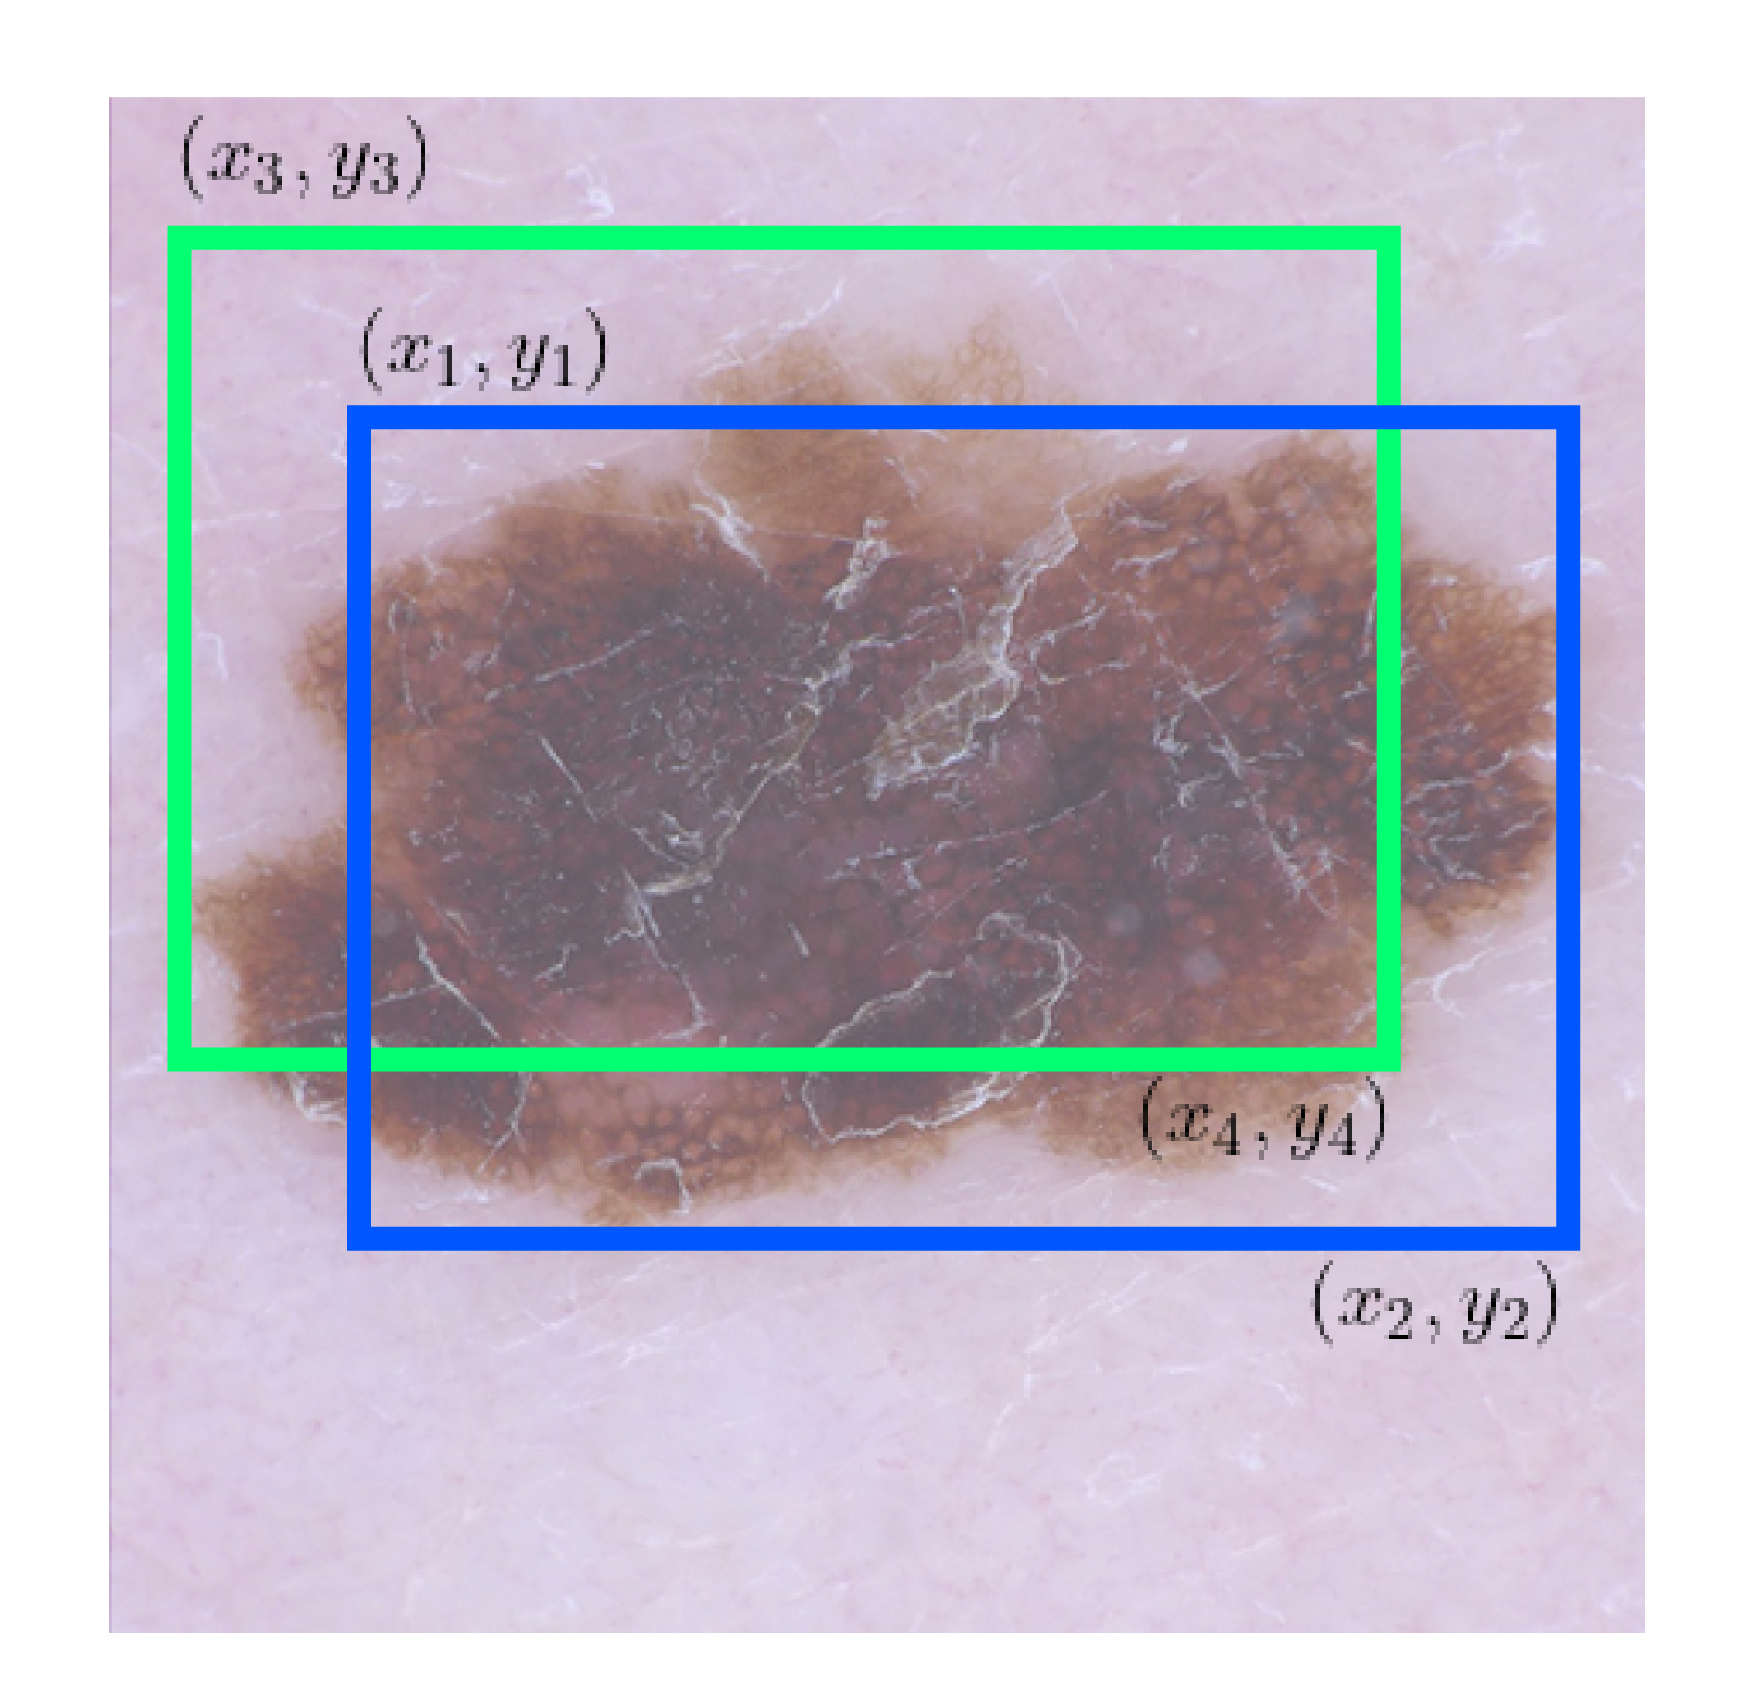
\includegraphics[width=3cm]{../img/IoU Original - Latex.png}
        &
        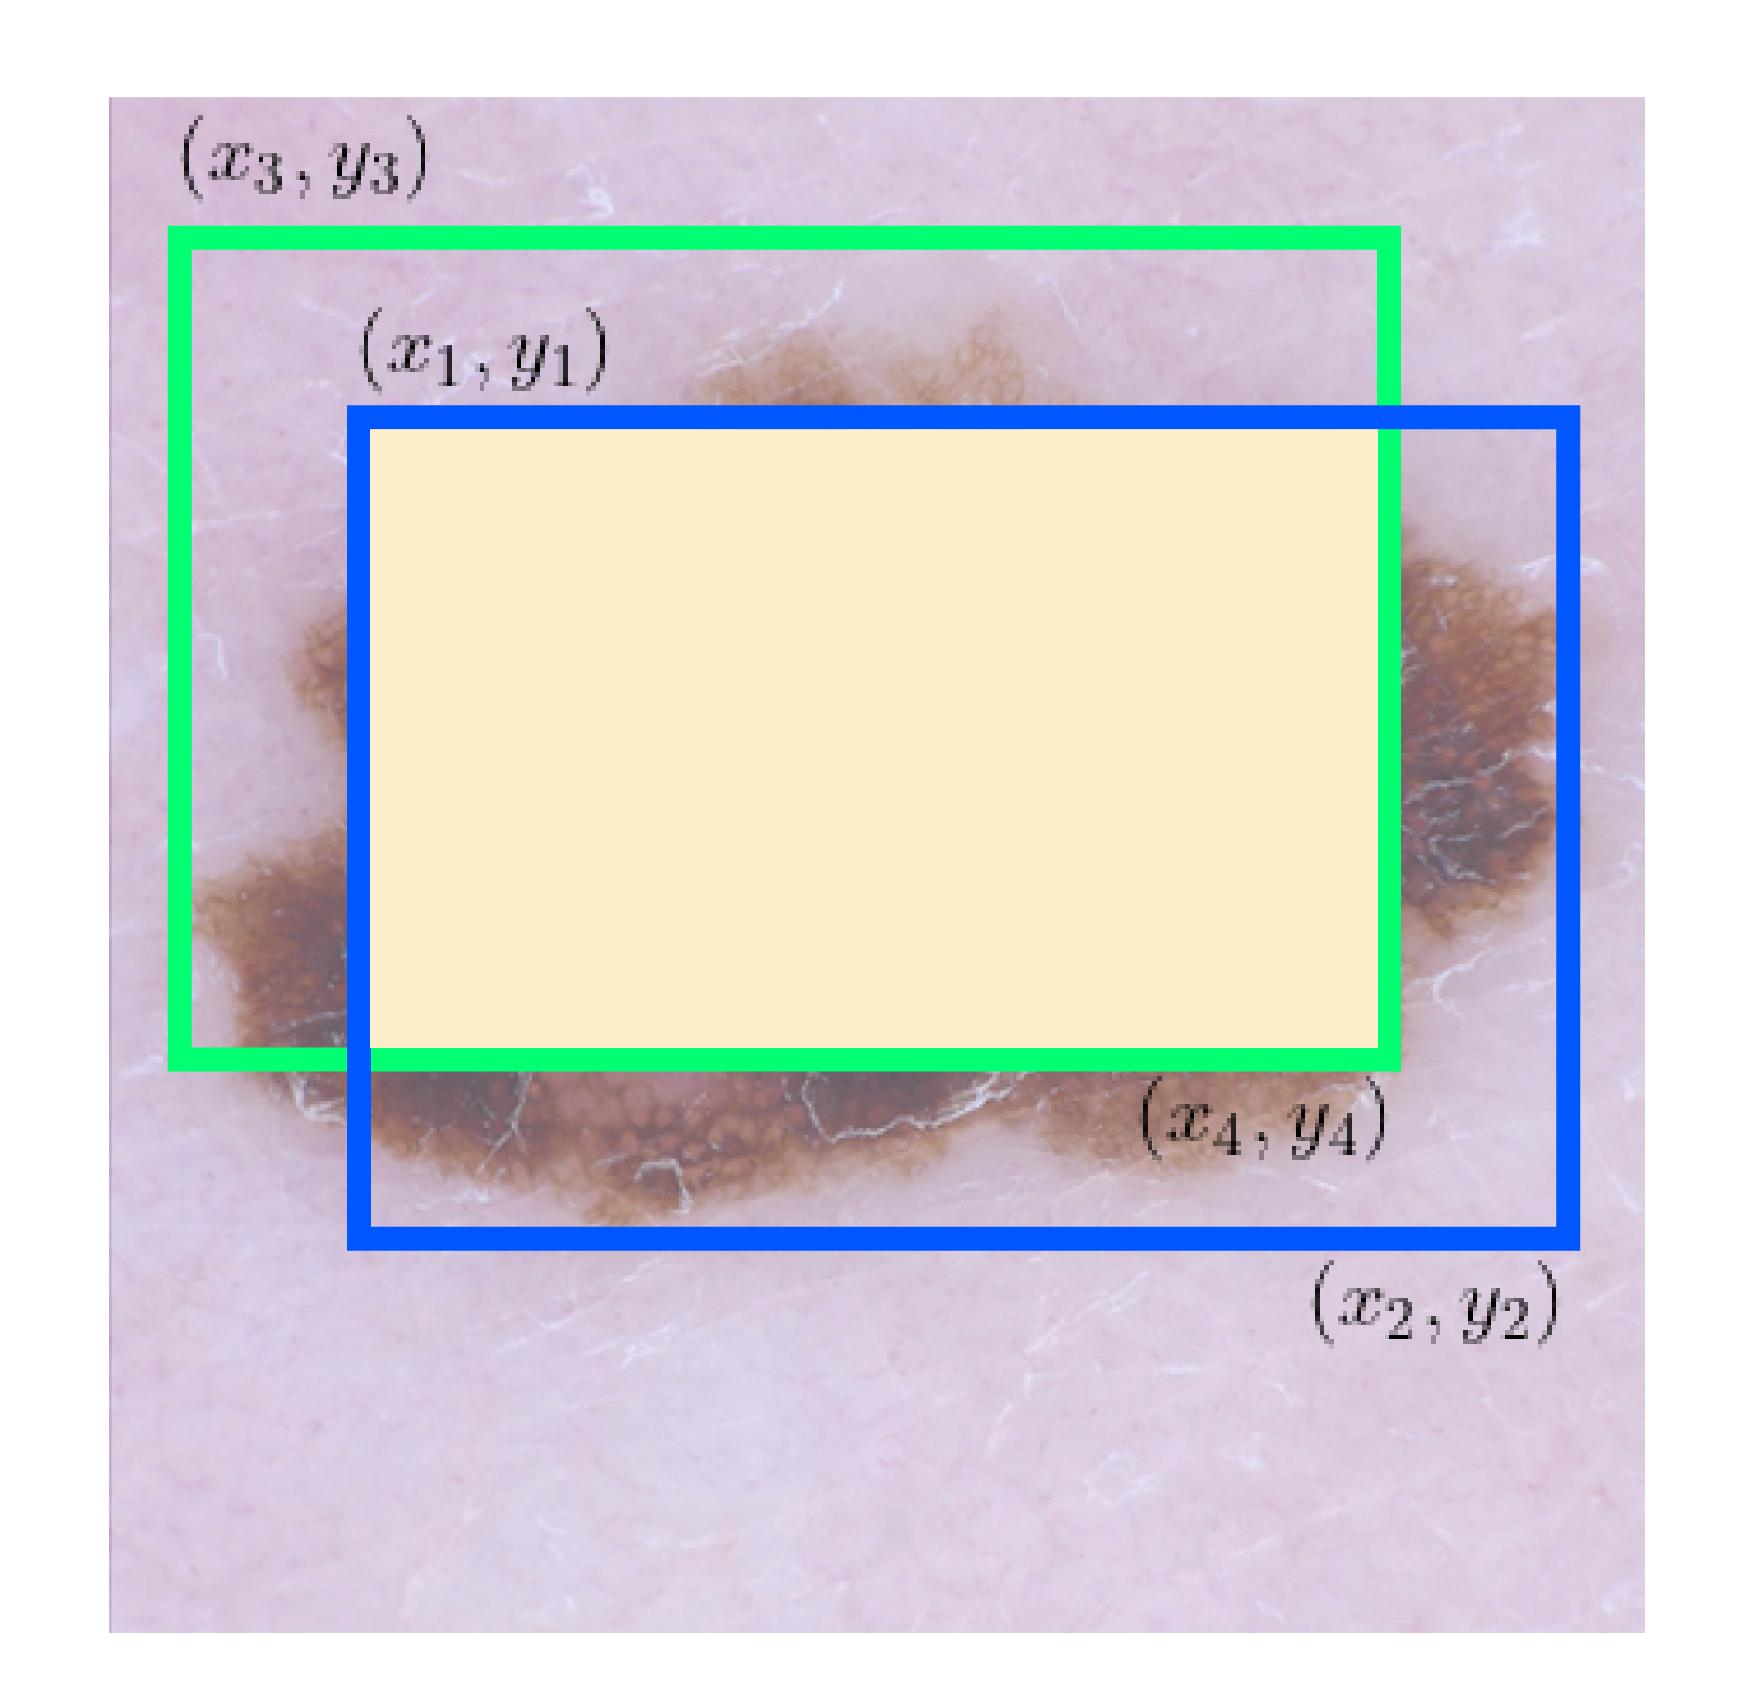
\includegraphics[width=3cm]{../img/IoU Overlapped - Latex.png}
        &
        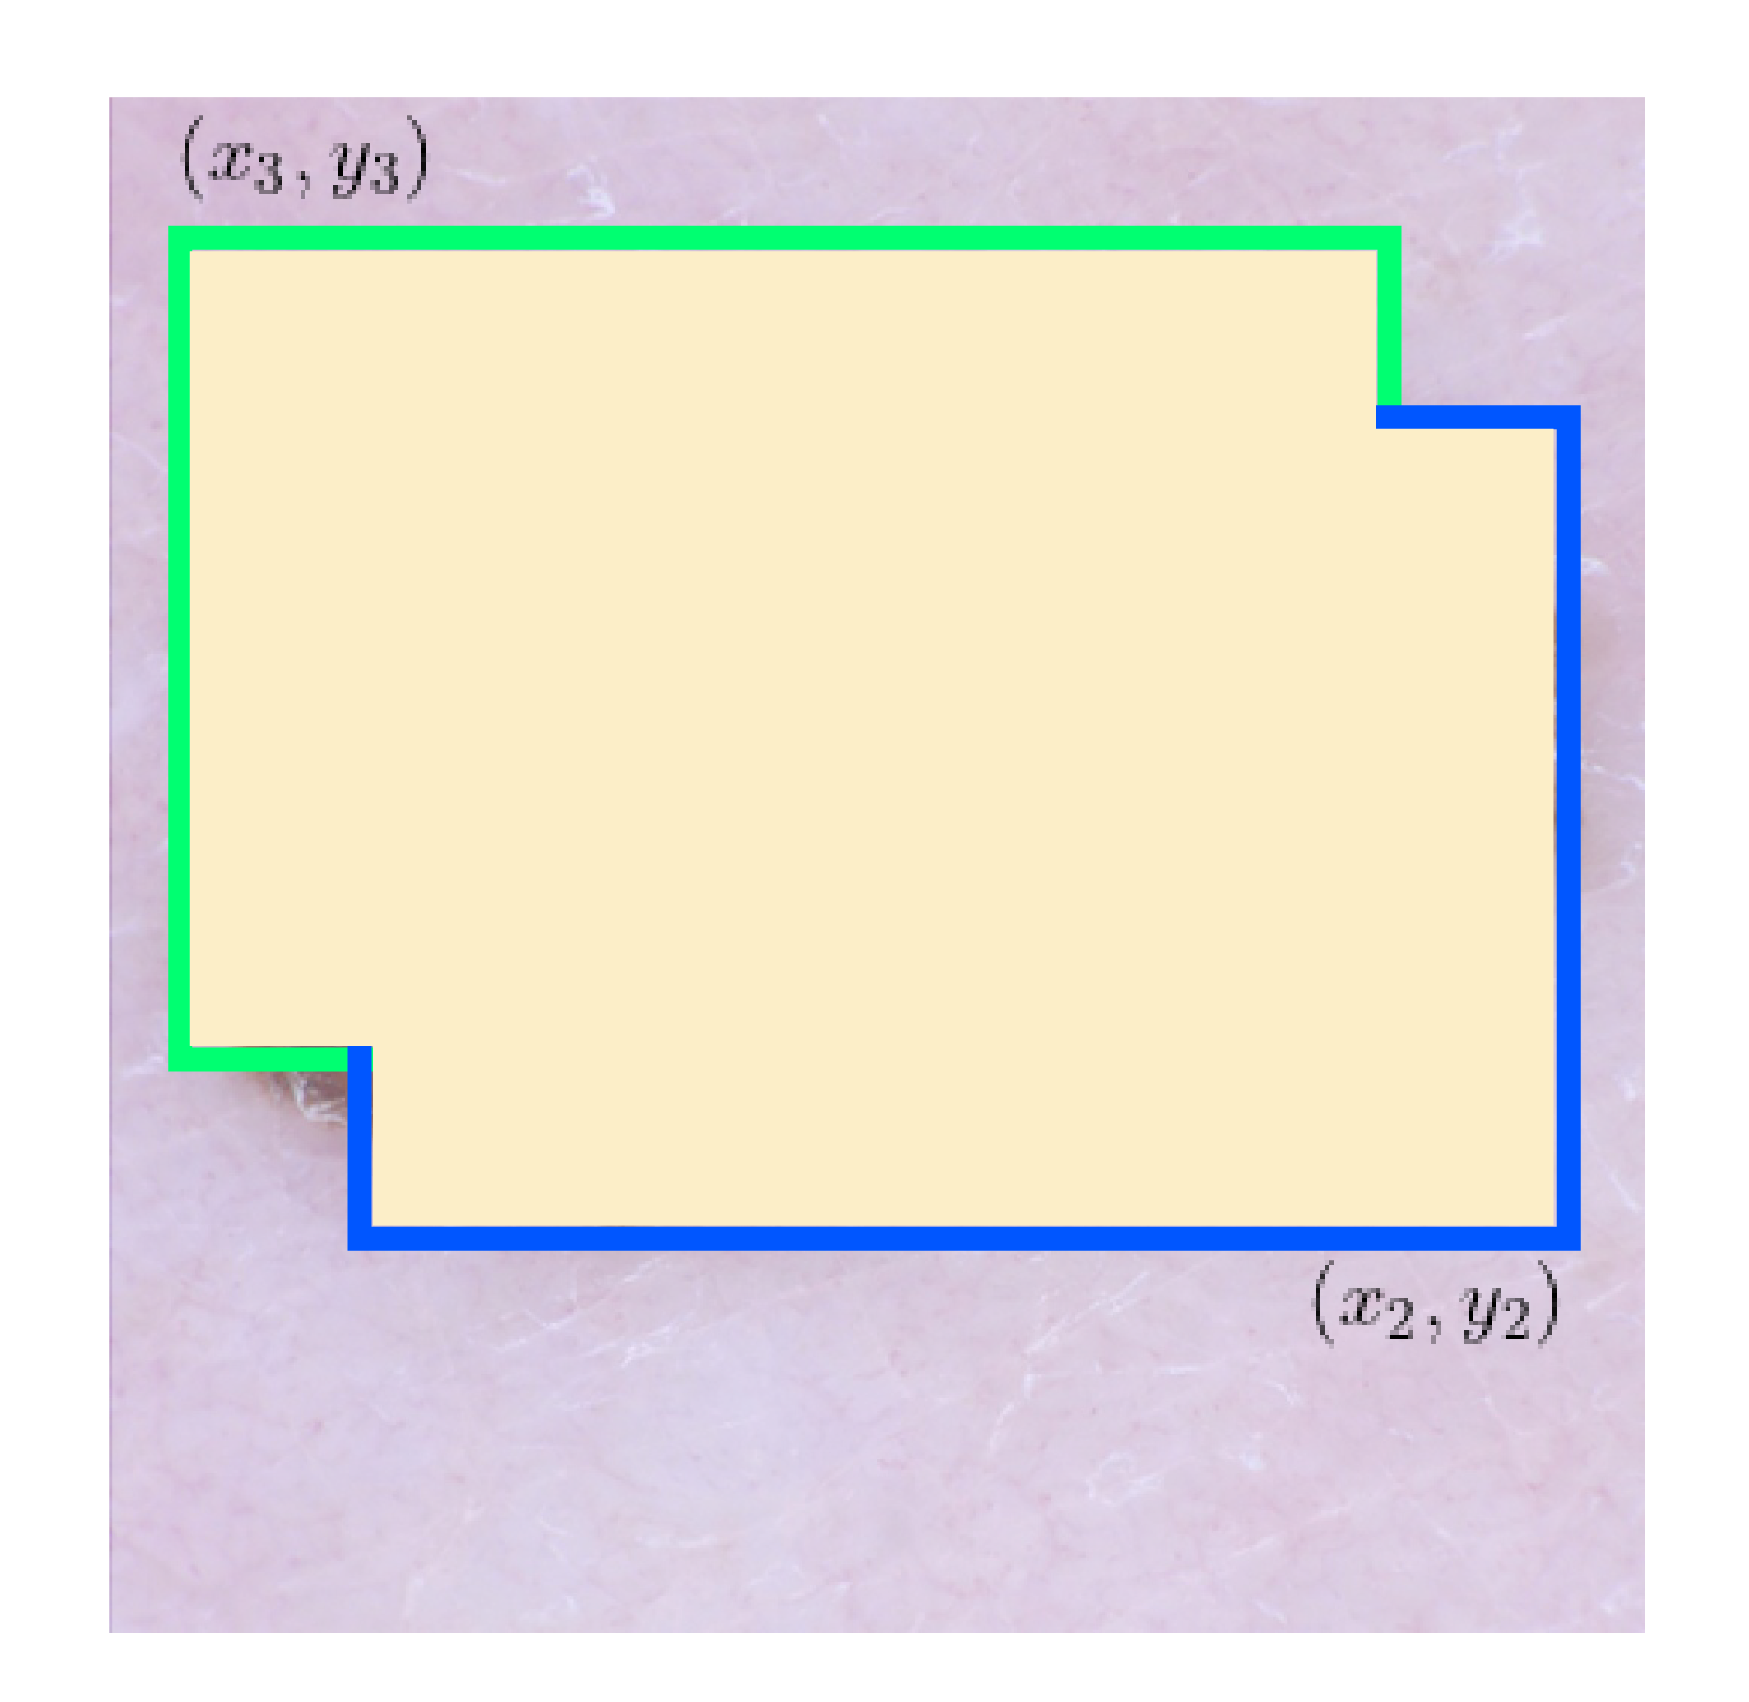
\includegraphics[width=3cm]{../img/IoU Union - Latex.png}\\
        (a) &(b) &(c)\\
    \end{tabular}
    \caption{Menunjukkan kondisi kotak pembatas (a) IoU; (b) \textit{Overlapped area}; (c) \textit{Union area}}
    \label{fig:iou-cond}
\end{figure}

Dari kedua kotak pembatas tersebut didapatkan dua bagian, yaitu \textit{overlap area} dan \textit{union area}. \textit{Overlap area} merupakan bagian tumpang tindih antara kotak pembatas data aktual dan kotak pembatas hasil prediksi. Sedangkan \textit{union area} merupakan gabungan antara kedua kotak pembatas. \textit{Overlap area} dan \textit{union area} seperti terlihat pada Gambar \ref{fig:iou-cond}. Pembagian antara \textit{overlap area} dengan \textit{union area} menghasilkan nilai IoU seperti pada Persamaan \ref{eq:iou}. Perhitungan \textit{overlap area} dan \textit{union area} seperti terlihat pada Persamaan \ref{eq:oa} dan \ref{eq:ua}. Nilai $x_a1, x_a2, y_a1, y_a2$ pada perhitungan tersebut didapatkan seperti pada Persamaan \ref{eq:xa1} - \ref{eq:ya2}.
\begin{align}
    \label{eq:xa1}
    x_{a1} &= max(x_1, x_3)\\
    \label{eq:xa2}
    x_{a2} &= max(x_2, x_4)\\
    \label{eq:ya1}
    y_{a1} &= max(y_1, y_3)\\
    \label{eq:ya2}
    y_{a2} &= max(y_2, y_4)\\
    \label{eq:oa}
    OA     &= (x_{a2}-x_{a1}\ast (y_{a2}-y_{a1}))\\
    \label{eq:ua}
    UA     &= (x_2-x_1)\ast (y_2-y_1) + (x_4-x_3)\ast (y_4-y_3) - OA\\
    \label{eq:iou}
    IoU    &= \frac{OA}{UA}
\end{align}

Dalam menentukan nilai IoU, sangat penting untuk memperhatikan ambang batas IoU. Karena hal ini akan menentukan kategori klasifikasi seperti pada Gambar \ref{fig:iou-cat}. Jika ambang batas IoU adalah $0.5$ maka Gambar \ref{fig:iou-cat} (a) termasuk ke dalam FP, Gambar \ref{fig:iou-cat} (b) dan (c) termasuk ke dalam TP. Sedangkan kondisi kotak pembatas data aktual dan kotak pembatas hasil prediksi tidak beririsan sama sekali dikategorikan sebagai FN.

\begin{figure}[H]
    \centering
    \begin{tabular}{ccc}
        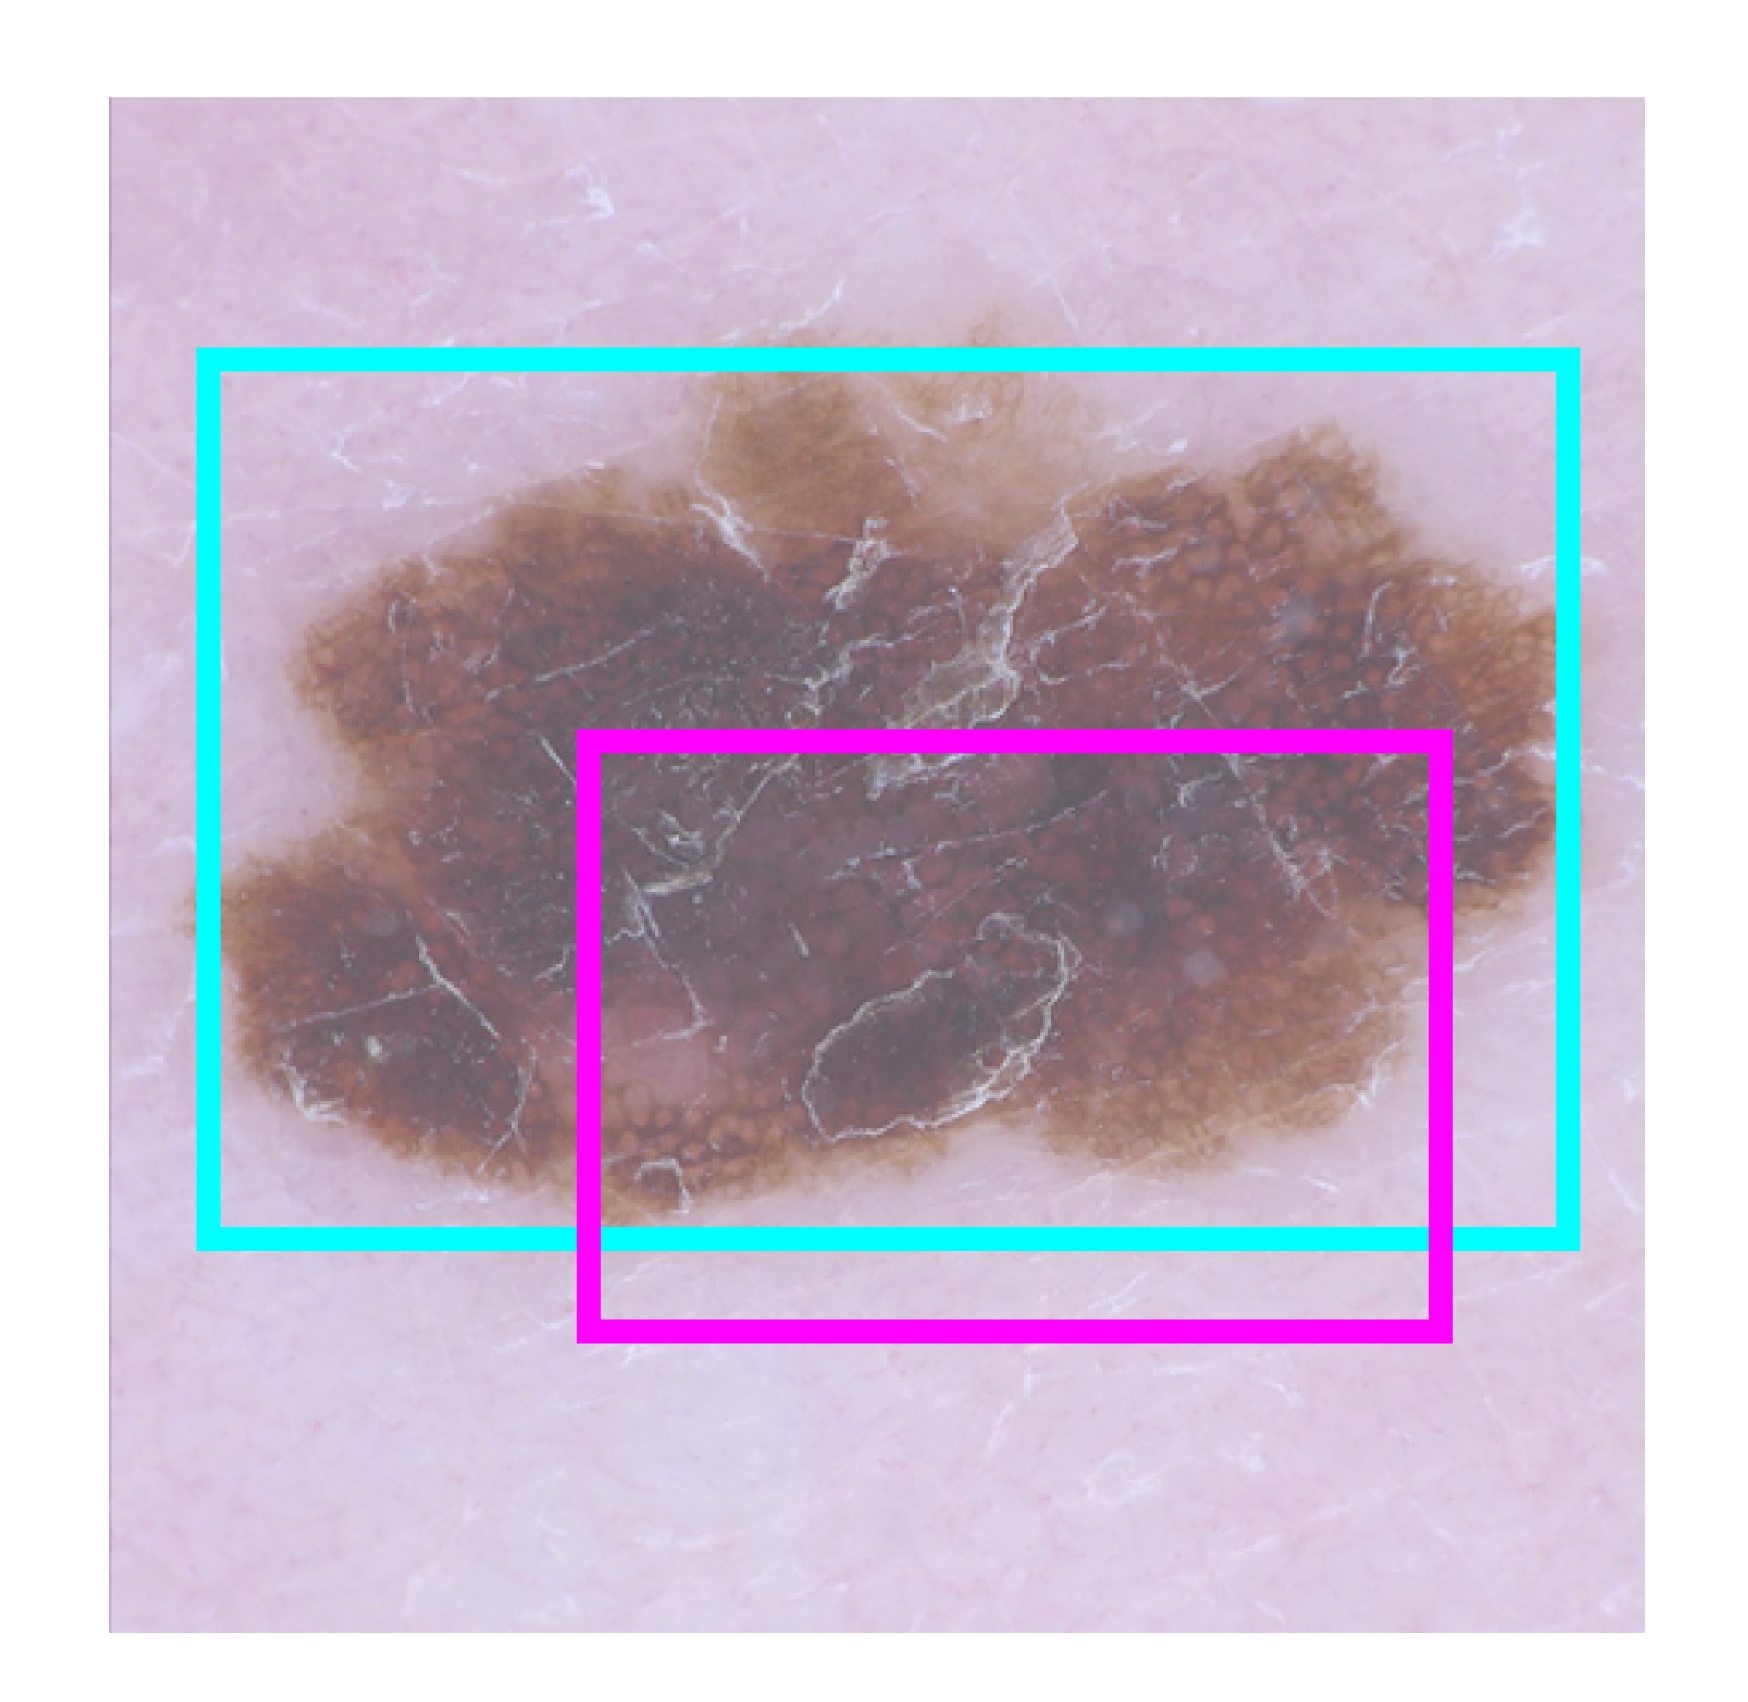
\includegraphics[width=2cm]{../img/IoU Poor - Latex.PNG}
        &
        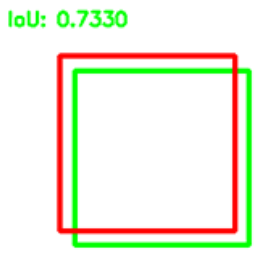
\includegraphics[width=2cm]{../img/IoU Good - Latex.PNG}
        &
        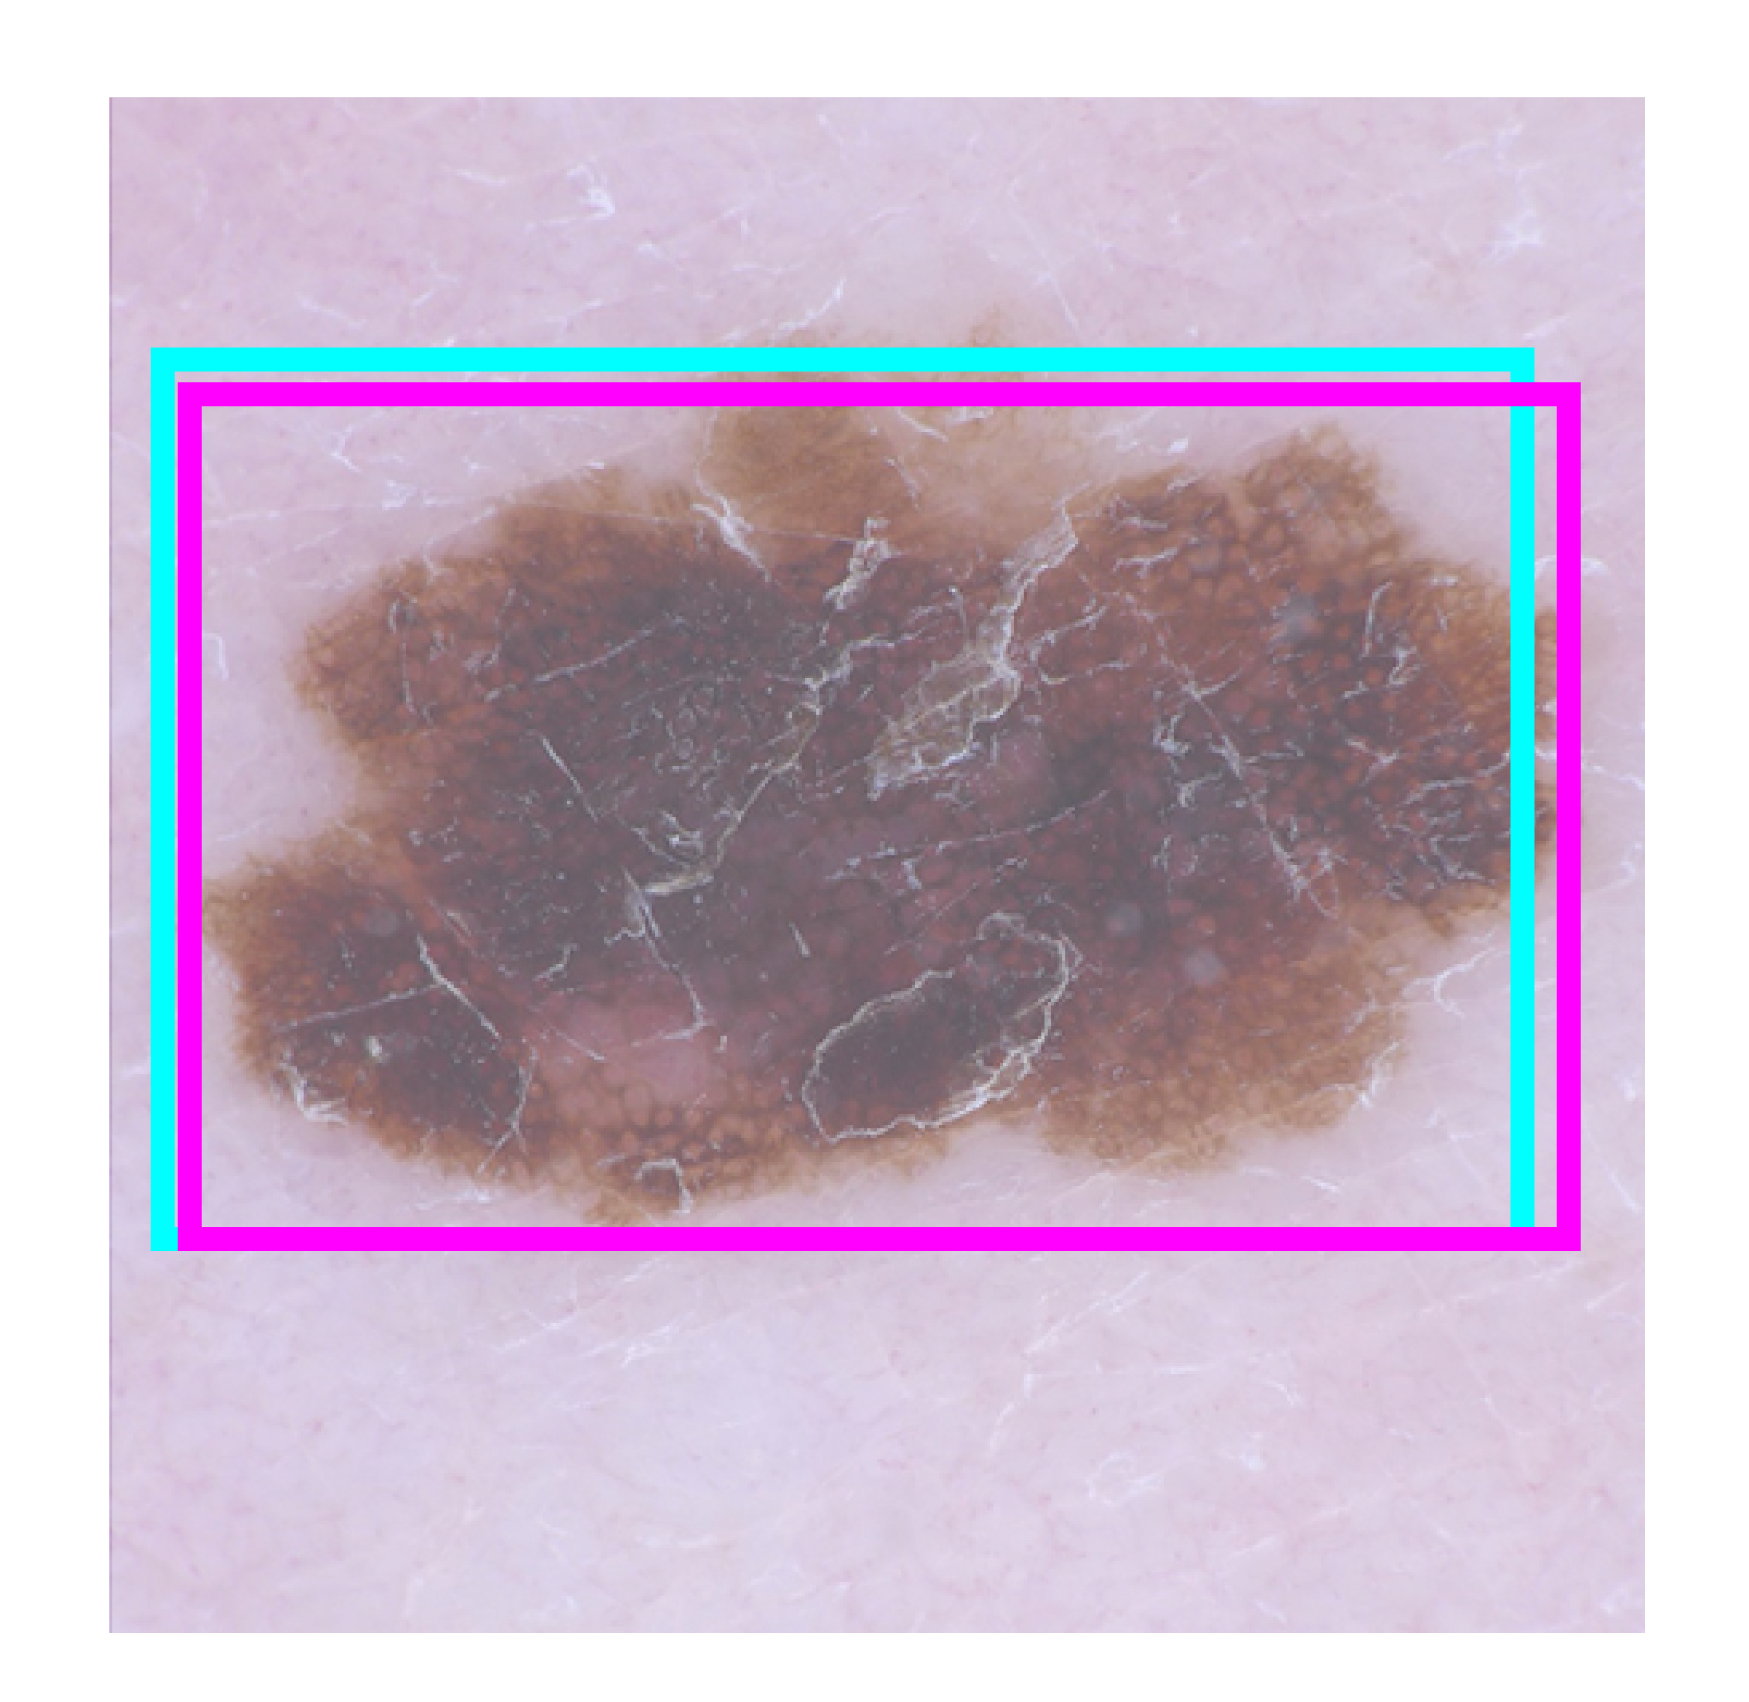
\includegraphics[width=2cm]{../img/IoU Excellent - Latex.PNG}\\
        (a) &(b) &(c)\\
    \end{tabular}
    \caption{Menunjukkan kondisi nilai IoU (a) Nilai IoU kurang baik; (b) Nilai IoU baik; (c) Nilai IoU sangat baik}
    \label{fig:iou-cat}
    Sumber: \citep{Cowton2019}
\end{figure}

\section{\textit{mean Average Precision} (mAP)}
mAP merupakan salah satu metode evaluasi model terutama pada model deteksi objek, seperti Fast R-CNN, MobileNet SSD, dan YOLO. Semakin baik model deteksi objek maka semakin tinggi nilai mAP. mAP menghitung rata-rata \textit{Average Precision} (AP) per kelas seperti terlihat pada Persamaan \ref{eq:map}. AP merupakan perhitungan \textit{precision} dan \textit{recall} pada setiap kelas seperti terlihat pada Persamaan \ref{eq:ap}. \textit{Precision} merupakan rasio antara kelas positif yang diprediksi dengan benar terhadap total data yang diklasifikasikan sebagai kelas positif. \textit{Recall} merupakan rasio antara kelas positif yang diprediksi dengan benar terhadap seluruh data positif. Perhitungan \textit{precision} dan \textit{recall} seperti terlihat pada Persamaan \ref{eq:precision} dan \ref{eq:recall} dimana $P$ dan $R$ merupakan \textit{precision} dan \textit{recall} \citep{Shultz2017}.
\begin{align}
    \label{eq:precision}
    P &= \frac{TP}{TP+FP}\\
    \label{eq:recall}
    R &= \frac{TP}{TP+FN}\\
    \label{eq:ap}
    AP &= \sum_{i=0}^{n-1} (R_i+R_{i+1})\ast P(i)\\
    \label{eq:map}
    mAP &= \frac{1}{n}\sum_{i=1}^{n} AP_i
\end{align}

\section{Integrasi Keislaman}
Kehidupan manusia di dunia tidak akan terlepas dari ujian. Bahkan, awal mula manusia di bumi karena ujian yang diberikan oleh Allah kepada Nabi Adam \textit{'alaihissalam}. Ujian dari Allah \textit{subhanallahu wa ta'ala} dapat berupa perkara yang disukai oleh manusia, seperti harta, tahta, dan wanita. Sedangkan perkara yang tidak disukai oleh manusia, seperti musibah, penyakit, dan kesengsaraan. Musibah dapat berupa bencana seperti musim paceklik yang akan menimpa suatu kaum pada masa Nabi Yusuf \textit{'alaihissalam} sebagaimana dalam firman-Nya:

\begin{flushright}
    \begin{RLtext}
        قَالَ تَزْرَعُوْنَ سَبْعَ سِنِيْنَ دَاَبًاۚ فَمَا حَصَدْتُّمْ فَذَرُوْهُ فِيْ سُنْۢبُلِهٖٓ اِلَّا قَلِيْلًا مِّمَّا تَأْكُلُوْنَ (٧٤) ثُمَّ يَأْتِيْ مِنْۢ بَعْدِ ذٰلِكَ سَبْعٌ شِدَادٌ يَّأْكُلْنَ مَا قَدَّمْتُمْ لَهُنَّ اِلَّا قَلِيْلًا مِّمَّا تُحْصِنُوْنَ (٨٤)
    \end{RLtext}
\end{flushright}

Artinya: "(Yusuf) berkata, 'Bercocoktanamlah kamu tujuh tahun berturut-turut! Kemudian apa yang kamu tuai, biarkanlah di tangkainya, kecuali sedikit untuk kamu makan. Kemudian, sesudah itu akan datang tujuh (tahun) yang sangat sulit (paceklik) yang menghabiskan apa yang kamu simpan untuk menghadapinya, kecuali sedikit dari apa (bibit gandum) yang kamu simpan." (Yusuf: 47-48). Nabi Yusuf \textit{'alaihissalam} memberitakan bahwa selama tujuh tahun musim paceklik itu tidak akan ada tumbuhan yang dapat hidup dan hasil panen akan gagal. Oleh sebab itu, Nabi Yusuf \textit{'alaihissalam} berkata kepada mereka, "... yang menghabiskan apa yang kalian simpan untuk menghidupinya (tahun sulit), kecuali sedikit dari (bibit gandum) yang kalian simpan". Imam Ibnu Katsir menafsirkan ayat ini dengan menjelaskan bahwa seseorang harus melakukan persiapan sebelum bencana terjadi sebagaimana penyakit yang akan menimpa. Jika muncul suatu kecurigaan atau muncul suatu pertanda dari penyakit dianjurkan untuk melakukan upaya pencegahan.

% TODO: Tuliskan ayat mengenai mitigasi

    \subsection{Hikmah Orang Sakit}
    Seorang mukmin tidak akan pernah terlepas dari tiga keadaan, yaitu jika mendapat nikmat maka ia bersyukur, jika mendapat susah maka ia bersabar, dan jika membuat dosa maka ia bertaubat. Hal ini merupakan kebahagiaan bagi seorang mukmin sebagaimana sabda Rasulullah \textit{shalallahu 'alaihi wa sallam}, 
    
    \begin{flushright}
        \begin{RLtext}
            عَجَبًا ِلأَمْرِ الْمُؤْمِنِ إنَّ أَمْرَهُ كُلَّهُ لَهُ خَيْرٌ وَلَيْسَ ذَلِكَ ِلأَحَدٍ إِلاَّ لْمُؤْمِنِ، إِنْ أَصَابَتْهُ سَرَّاءُ شَكَرَ فَكَانَ خَيْرًا لَهُ، وَإِنْ أَصَابَتْهُ ضَرَّاءُ صَبَرَ فَكَانَ خَيْراً لَهُ
        \end{RLtext}
    \end{flushright}

    Artinya: "Sungguh menakjubkan perkara seorang mukmin, sesungguhnya semua urusannya merupakan kebaikan, dan hal ini tidak terjadi kecuali bagi orang mukmin. Jika dia mendapat kegembiraan, maka dia bersyukur dan itu merupakan kebaikan baginya, dan jika mendapat kesusahan, maka dia bersabar dan ini merupakan kebaikan baginya." (HR. Muslim: 2999). Ketika seorang mukmin mendapatkan nikmat dan bersyukur maka akan mendapatkan kebaikan dari Allah \textit{subhanallahu wa ta'ala}. Sedangkan ketika seorang mukmin mendapat kesusahan dan bersabar maka akan mendapatkan kebaikan pula dari Allah \textit{subhanallahu wa ta'ala}.

    Penyakit merupakan salah satu jalan untuk mendapatkan ampunan dosa dari Allah \textit{subhanallahu wa ta'ala}. Namun, terdapat ketentuan untuk mendapatkan pengampunan dosa ketika sakit, seperti tidak menjalankan maksiat ketika sakit atau tetap dalam ketakwaan ketika sakit. Rasulullah \textit{shalallahu 'alaihi wa sallam} bersabda terkait seorang mukmin yang sakit, "Tidaklah menimpa seorang mukmin rasa sakit yang terus menerus, kepayahan, penyakit, dan juga kesedihan, bahkan sampai kesusahan yang menyusahkannya, melainkan akan dihapuskan dengannya dosa-dosanya." (HR. Muslim). Di sisi lain, penyakit juga merupakan peringatan dan hukuman dari apa yang telah diperbuat sebagaimana firman Allah \textit{subhanallahu wa ta'ala} dalam surat asy-Syura ayat 30,

    \begin{flushright}
        \<وَمَآ اَصَابَكُمْ مِّنْ مُّصِيْبَةٍ فَبِمَا كَسَبَتْ اَيْدِيْكُمْ وَيَعْفُوْا عَنْ كَثِيْرٍۗ (٠٣)>
    \end{flushright}

    Artinya: "Dan apa saja musibah yang menimpamu maka adalah disebabkan oleh perbuatan tanganmu sendiri, dan Allah memaafkan sebagian besar (dari kesalahan-kesalahanmu)." (asy-Syura: 30).

    \subsection{Ikhtiar Orang Sakit}
    Tiap-tiap orang yang sakit pasti menginginkan kesembuhan. Bagi orang sakit, usaha untuk sembuh merupakan keharusan karena dapat mengganggu ketakwaan kepada Allah \textit{subhanallahu wa ta'ala} jika sakit tidak segera dihilangkan. Syaikh Muhammad bin Shalih al-'Utsaimin \textit{rahimahullah} mengatakan bahwa ikhtiar untuk mendapatkan kesembuhan bagi orang sakit adalah suatu keharusan karena jika ditinggalkan dapat membahayakan tubuh. Hal ini mempertimbangkan fungsionalitas tubuh sebagai sarana beribadah kepada Allah \textit{subhanallahu wa ta'ala}. Misalnya ketika seseorang terkena penyakit kanker maka usaha untuk menghilangkan kanker tersebut harus dilakukan. Jika hal tersebut tidak dilakukan maka kanker akan menyebar ke jaringan tubuh lain dan menimbulkan penyakit baru. Oleh karena itu, menghilangkan kanker yang membahayakan merupakan suatu keharusan bagi seorang mukmin. Rasulullah \textit{shalallahu 'alaihi wa sallam} memerintahkan kepada umatnya untuk mencari kesembuhan dan tidak berputus asa dari atas suatu penyakit yang dideritanya. Dari Jabir bin 'Abdillah, Rasulullah \textit{shalallahu 'alaihi wa sallam} bersabda,

    \begin{flushright}
        \<لِكُلِّ دَاءٍ دَوَاءٌ فَإِذَا أُصِيبَ دَوَاءُ الدَّاءِ بَرَأَ بِإِذْنِ اللَّهِ عَزَّ وَجَلَّ>
    \end{flushright}

    Artinya: “Setiap penyakit itu pasti ada obatnya. Oleh karena itu, barang siapa yang tepat dalam melakukan pengobatan suatu penyakit, maka dengan izin Allah ‘azza wa  jalla dia akan sembuh.” (HR. Muslim, Ibn Hiban, dan Hakim). Dari Abu Hurairah \textit{radhiallahu 'anhu}, dia mengabarkan bahwa Rasulullah \textit{shalallahu 'alaihi wa sallam} bersabda,

    \begin{flushright}
        \<ما أنْزَلَ اللَّهُ داءً إلَّا أنْزَلَ له شِفاءً>
    \end{flushright}

    “Tidaklah Allah menurunkan suatu penyakit, melainkan Dia turunkan obat untuknya.” (HR. Ibn Majah dan dishahihkan al-Albani).

    Berdasarkan pemaparan di atas, kanker kulit merupakan salah satu bentuk penyakit yang harus disembuhkan karena jika diabaikan dapat membahayakan jaringan tubuh di sekitarnya. Salah satu usaha untuk mendapatkan kesembuhan dari kanker kulit adalah melakukan diagnosis kanker kulit. Penelitian ini melakukan diagnosis kanker kulit dengan metode YOLO-v7 untuk mengetahui jenis kanker kulit yang diderita sehingga dapat meminimalisir resiko yang terjadi akibat kanker kulit.








